\subsection{The Galois group of the algebraic closure of a finite field}

Let \(S \neq \{1\}\) be a set of integers \(\geqslant 1\) stable under multiplication; we shall order it by the relation « \(m\) divides \(n\) ». When \(m\) divides \(n\) , we have \(mZ \supset nZ\) , hence there is a canonical homomorphism \(\pi_{m,n}\) of the ring \(Z/nZ\) onto the ring \(Z/mZ\) . We denote by \(A(S)\) the inverse limit of the inverse system of rings \((Z/mZ, \pi_{m,n})\) indexed by \(S\) . Each finite set \(Z/mZ\) is equipped with the discrete topology and \(A(S)\) with the topology induced by that of the product \(\prod_{n \in S} (Z/nZ)\) .

Then A(S) is a compact topological ring (Gen.~Top. I, p.~64, Prop. 8). We see at once that the unique ring homomorphism \(\varphi\) of \(\mathbf{Z}\) into A(S) is injective with a dense image; we shall identify \(\mathbf{Z}\) with its image under \(\varphi\) in A(S). For the topology induced on \(\mathbf{Z}\) by that of A(S), the sets \(m\mathbf{Z}\) (for \(m \in S\) ) form a base of neighbourhoods of 0.

When \(S = N^{*}\) , \(A(S)\) is written \(\hat{Z}\) . When S consists of the powers of a prime number l, \(A(S)\) is written \(Z_{l}\) and is called « ring of l-adic integers ». We thus have

\[
\hat {\mathbf {Z}} = \varprojlim_ {m \geqslant 1} \mathbf {Z} / m \mathbf {Z}, \quad \mathbf {Z} _ {l} = \varprojlim_ {n \geqslant 0} \mathbf {Z} / l ^ {n} \mathbf {Z}.
\]

When S and T are two sets of integers stable under multiplication such that \(S \supset T\) , we have a natural projection \(\mathbf{A}(\mathbf{S}) \to \mathbf{A}(\mathbf{T})\) which is a continuous homomorphism of topological rings. In particular, for every prime number l we have a continuous homomorphism \(\hat{Z} \to Z_{l}\) . From it we obtain a continuous homomorphism

\[
\hat {\mathbf {Z}} \rightarrow \prod_ {l} \mathbf {Z} _ {l}
\]

(product extended over all prime numbers) ; this is an isomorphism of topological rings, as follows from the passage to the inverse limit in I, p.~112, Prop. 11.

Let K be a finite field of q elements and \(\bar{K}\) an algebraic closure of K. For every integer \(m \geqslant 1\) we denote by \(K_{m}\) the unique subfield of \(\bar{K}\) which is of degree m over K (Prop. 3). We have \(\bar{K} = \bigcup_{m \geqslant 1} K_{m}\) . Further we denote by \(\sigma_{q}\) the automorphism

\(x \mapsto x^{q}\) of the perfect field \(\bar{K}\) ; it is called the Frobenius automorphism of \(\bar{K}\) (relative to K).

PROPOSITION 5. --- There exists a unique isomorphism of topological groups \(\pi_{\mathbf{K}}: \hat{\mathbf{Z}} \to \operatorname{Gal}(\bar{\mathbf{K}} / \mathbf{K})\) such that \(\pi_{\mathbf{K}}(1) = \sigma_q\) .

Let \(\Gamma\) be the subgroup of \(\operatorname{Gal}(\bar{\mathbf{K}} / \mathbf{K})\) generated by \(\sigma_q\) . For every integer \(m > 0\) we have \(\sigma_q^m (x) = x^{q^m}\) for all \(x\in \bar{\mathbf{K}}\) , hence the set of fixed points of \(\sigma_q^m\) is equal to \(\mathbf{K}_m\) . Since \(\mathbf{K}_m\neq \bar{\mathbf{K}}\) , we have \(\sigma_q^m\neq 1\) . Hence there is an isomorphism \(\pi_0\) of \(\mathbf{Z}\) onto \(\Gamma\) which maps 1 to \(\sigma_q\) .

The field of invariants of \(\Gamma\) consists of the \(x \in \bar{K}\) such that \(x^{q} = x\) , hence is equal to K. Therefore (V, p.~67, Lemma 2) the group \(\Gamma\) is dense in \(\operatorname{Gal}(\bar{\mathbf{K}}/\mathbf{K})\) . Since every subextension of \(\bar{K}\) of finite degree over K is one of the fields \(K_{m}\) , the subgroups \(\operatorname{Gal}(\bar{\mathbf{K}}/\mathbf{K}_{m})\) form a fundamental system of neighbourhoods of 1 in \(\operatorname{Gal}(\bar{\mathbf{K}}/\mathbf{K})\) . It is clear that \(\Gamma \cap \operatorname{Gal}(\bar{\mathbf{K}}/\mathbf{K}_{m})\) is the cyclic group generated by \(\sigma_{q}^{m}\) , hence equal to \(\pi_{0}(m\mathbf{Z})\) .

From the above remarks about the topology of \(\hat{Z}\) the isomorphism \(\pi_{0}:Z\to\Gamma\) extends in a unique fashion to an isomorphism of topological groups \(\pi_{K}:\hat{Z}\to\operatorname{Gal}(\bar{\mathbf{K}}/\mathbf{K})\) .

Let \(m \geqslant 1\) be an integer; it is clear that the Frobenius automorphism of \(\bar{\mathbf{K}}\) relative to \(\mathbf{K}_m\) is \(\sigma_q^m\) . Hence we obtain the relation

\[
\pi_ {\mathrm{K} _ {m}} (a) ^ {*} = \pi_ {\mathrm{K}} (m a) \quad \text { for } \quad a \in \hat {\mathbf {Z}}.\tag{5}
\]

\subsection{Cyclotomic polynomials over a finite field}

Let K be a finite field of q elements, \(n \geqslant 1\) an integer not divisible by the characteristic p of K and \(R_{n}\) a cyclotomic extension of level n of K (V, p.~81). We know that the group \(\mu_{n}(R_{n}) = \mu_{n}\) of n-th roots of unity in \(R_{n}\) is cyclic of order n, that \(R_{n} = K(\mu_{n})\) and that there exists an injective homomorphism

\[
\varphi_ {n}: \operatorname{Gal} \left(\mathrm{R} _ {n} / \mathrm{K}\right)\rightarrow (\mathbf {Z} / n \mathbf {Z}) ^ {*}
\]

such that \(\sigma(\zeta) = \zeta^j\) for \(\sigma \in \operatorname{Gal}(\mathbf{R}_n / \mathbf{K})\) , \(\zeta \in \mu_n\) and \(j \in \varphi_n(\sigma)\) .

Further, if \(f\) is the degree of \(\mathbf{R}_n\) over \(\mathbf{K}\) , then the Galois group of \(\mathbf{R}_n\) over \(\mathbf{K}\) is cyclic of order \(f\) , generated by the automorphism \(\sigma_q: x \mapsto x^q\) (V, p.~95, Prop. 4). We have at once:

PROPOSITION 6. --- The image under \(\varphi_{n}\) of the Frobenius automorphism \(\sigma_{q}\) is the residue class of \(q\) mod \(n\) .

Therefore, taking into account Prop. 6 of V, p.~84 :

COROLLARY. --- The degree of \(R_{n}\) over K is the least integer \(f \geqslant 1\) such that \(q^{f} \equiv 1 \pmod{n}\) . For the cyclotomic polynomial \(\Phi_{n}\) to be irreducible over K it is necessary and sufficient that the group \((\mathbf{Z}/n\mathbf{Z})^{*}\) should be generated by the residue class of q modulo n.

Examples. --- 1) The polynomial \(\Phi_3(\mathbf{X}) = \mathbf{X}^2 + \mathbf{X} + 1\) is irreducible in \(\mathbf{F}_q[\mathbf{X}]\) if and only if \(q \equiv 2 \pmod{3}\) . Likewise \(\Phi_4(\mathbf{X}) = \mathbf{X}^2 + 1\) is irreducible in \(\mathbf{F}_q[\mathbf{X}]\) if and only if \(q \equiv 3 \pmod{4}\) and for \(\Phi_5 = \mathbf{X}^4 + \mathbf{X}^3 + \mathbf{X}^2 + \mathbf{X} + 1\) , the irreducibility condition reads \(q \equiv 2, 3 \pmod{5}\) .

\begin{enumerate}
\def\labelenumi{\arabic{enumi})}
\setcounter{enumi}{1}
\tightlist
\item
  We have \(5^2 \equiv 1 \pmod{12}\) , hence the residue class of 5 (mod 12) does not generate \((\mathbf{Z}/12\mathbf{Z})^*\) . So the polynomial \(\Phi_{12}(\mathbf{X}) = \mathbf{X}^4 - \mathbf{X}^2 + 1\) is not irreducible in \(\mathbf{F}_5[\mathbf{X}]\) ; in fact we have
\end{enumerate}

\[
\Phi_ {12} (\mathbf {X}) = \left(\mathbf {X} ^ {2} + 2 \mathbf {X} - 1\right) \left(\mathbf {X} ^ {2} - 2 \mathbf {X} - 1\right)
\]

in \(\mathbf{F}_5[\mathbf{X}]\) .

\section{p-RADICAL EXTENSIONS OF HEIGHT ≤ 1}

Throughout this paragraph \(p\) denotes a prime number. All the fields considered are of characteristic \(p\) .

\subsection{\texorpdfstring{\(p\)-free subsets and \(p\)-bases}{p-free subsets and p-bases}}

DEFINITION 1. --- Let K be a field and L a p-radical extension of height ≤1 of K. A family \((x_i)_{i \in I}\) of elements of L is said to be p-free over K (resp. a p-basis of L over K) if \(x_i \notin K\) for all \(i \in I\) and the homomorphism of \(\otimes_{i \in I} K(x_i)\) into L

derived from the canonical injections \(u_{i}:\mathbf{K}(x_{i})\to \mathbf{L}\) is injective (resp. bijective).

If \(a\) is an element of \(\mathbf{L} - \mathbf{K}\) , it is \(p\) -radical of height 1, and so its minimal polynomial over \(\mathbf{K}\) is \(\mathbf{X}^p - a^p\) (V, p.~24, Prop. 1); therefore \(\{1, a, \ldots, a^{p-1}\}\) is a basis of \(\mathbf{K}(a)\) over \(\mathbf{K}\) . Let \((x_i)_{i \in I}\) be a family of elements of \(\mathbf{L} - \mathbf{K}\) and \(\Lambda\) the subset of \(\mathbf{N}^{(I)}\) consisting of all families of finite support \(\alpha = (\alpha_i)_{i \in I}\) such that \(\alpha_i < p\) for all \(i \in I\) ; Prop. 9 (III, p.~471) shows that the elements \(\otimes_{i \in I} x_i^{\alpha_i}\) as \(\alpha\) runs

over \(\Lambda\) form a basis of the vector space \(\otimes_{i\in I}\mathbf{K}(x_i)\) over \(\mathbf{K}\) . Moreover, the canonical

homomorphism of \(\otimes_{i\in I}\mathbf{K}(x_i)\) into \(L\) has as image \(\mathbf{K}(x_i)_{i\in I}\) (V, p.~18, Cor. 1), we

thus have the following proposition :

PROPOSITION 1. --- Let K be a field, L a p-radical extension of height ≤1 of K and \(\mathbf{x} = (x_{i})_{i \in I}\) a family of elements of L. Then the vector space \(\mathrm{K}(x_{i})_{i \in I}\) over K is generated by the products \(x^{\alpha} = \prod_{i \in I} x_{i}^{\alpha_{i}}\) for \(\alpha\) in \(\Lambda\) . For

\((x_{i})_{i\in I}\) to be \(p\) -free (resp. a \(p\) -basis) it is necessary and sufficient that the family \((\mathbf{x}^{\alpha})_{\alpha \in \Lambda}\) should be free over \(\mathbf{K}\) (resp. a basis of \(\mathbf{L}\) over \(\mathbf{K}\) ).

COROLLARY. --- Let L' be an extension of a field K, generated by two linearly disjoint subextensions K' and L. Suppose that L is p-radical of height \(\leqslant 1\) over K; then L' is p-radical of height \(\leqslant 1\) over K'. Moreover, for a family of elements of L to be p-free over K (resp. a p-basis of L over K) it is necessary and sufficient that it should be p-free over K' (resp. a p-basis of L' over K').

We have \(L^{p} \subset K \subset K'\) and \(L' = K'(L)\) , whence \(L'^{p} = K'^{p}(L^{p}) \subset K'\) . In other words, \(L'\) is a p-radical extension of height \(\leqslant 1\) of \(K'\) . The other assertions of the corollary follow at once from Prop. 1 and from V, p.~14, Prop. 5.

Remark. --- Let K be a field, L a p-radical extension of height \(\leqslant1\) of K and \((x_{i})_{i\in I}\) a family of elements of L. Let A be the polynomial algebra \(\mathrm{K}[(\mathrm{X}_{i})_{i\in I}]\) , a the ideal of A generated by the polynomials \(X_{i}^{p}-x_{i}^{p}\) and \(\varphi:A\to L\) the K-algebra homomorphism such that \(\varphi(\mathrm{X}_{i})=x_{i}\) for each \(i\in I\) . The family \((x_{i})_{i\in I}\) is p-free if and only if the kernel of \(\varphi\) is equal to a. For \(\mathrm{K}[(\mathrm{X}_{i})]/\mathfrak{a}\) may be identified with the algebra \(\otimes\mathrm{K}[\mathrm{X}_{i}]/(\mathrm{X}_{i}^{p}-x_{i}^{p})\) .

Let L be a p-radical extension of height \(\leqslant1\) of the field K. A subset S of L is said to be p-free (resp. a p-basis) if the family defined by the identity mapping of S onto itself is p-free (resp. a p-basis). For a family \((x_{i})_{i\in I}\) of elements of L to be p-free (resp. a p-basis) it is necessary and sufficient that the mapping \(i\mapsto x_{i}\) should be a bijection of I on a p-free subset (resp. a p-basis) of L. By Prop. 1, every subset of a p-free set is p-free; conversely, if S is a subset of L all of whose finite subsets are p-free, then S is p-free. Finally, a p-basis of L over K is a p-free subset B such that \(\mathrm{L}=\mathrm{K}(\mathrm{B})\) .

PROPOSITION 2. --- Let K be a field, L a p-radical extension of height ≤1 of K and S a subset of L. For S to be p-free it is necessary and sufficient that K(T) ≠ K(S) for every subset T ≠ S of S.

Suppose first that S is p-free and let \(T \neq S\) be a subset of S. Denote by \(\Lambda\) the set of families with finite support \(\alpha = (\alpha_{s})_{s \in S}\) of integers between 0 and p - 1; let \(\Lambda'\) be the subset of \(\Lambda\) consisting of the families \(\alpha = (\alpha_{s})_{s \in S}\) such that \(\alpha_{s} = 0\) for all s in S - T. We also put \(u_{\alpha} = \prod_{s \in S} s^{\alpha_{s}}\) for \(\alpha \in \Lambda\) . Then (V, p.~98,

Prop. 1) the family \((u_{\alpha})_{\alpha \in \Lambda}\) is a basis of \(\mathbf{K}(\mathbf{S})\) over \(\mathbf{K}\) and the subfamily \((u_{\alpha})_{\alpha \in \Lambda'}\) is a basis of \(\mathbf{K}(\mathbf{T})\) over \(\mathbf{K}\) . Since \(\Lambda' \neq \Lambda\) , we have \(\mathbf{K}(\mathbf{T}) \neq \mathbf{K}(\mathbf{S})\) .

Suppose now that S is not \(p\) -free. Then there exists an integer \(n \geqslant 1\) and a sequence of elements \(x_1, \ldots, x_n\) of S such that \((x_1, \ldots, x_{n-1})\) is \(p\) -free but \((x_1, \ldots, x_n)\) is not. We have \([\mathbf{K}(x_1, \ldots, x_{n-1}) : \mathbf{K}] = p^{n-1}\) and \([\mathbf{K}(x_1, \ldots, x_n) : \mathbf{K}] < p^n\) . Since \([\mathbf{K}(x_1, \ldots, x_n) : \mathbf{K}]\) is a multiple of \([\mathbf{K}(x_1, \ldots, x_{n-1}) : \mathbf{K}]\) , we thus have

\[
[ \mathrm{K} (x _ {1}, \dots , x _ {n}): \mathrm{K} ] = [ \mathrm{K} (x _ {1}, \dots , x _ {n - 1}): \mathrm{K} ].
\]

whence \(x_{n} \in \mathbf{K}(x_{1}, \ldots, x_{n-1})\) . This shows that \(\mathbf{K}(\mathbf{S} - \{x_{n}\}) = \mathbf{K}(\mathbf{S})\) .

PROPOSITION 3. --- Let K be a field, L a p-radical extension of height ≤1 of K and S, T two subsets of L. The following conditions are equivalent :

\begin{enumerate}
\def\labelenumi{\alph{enumi})}
\item
  The subset \(\mathbf{S}\) is \(p\) -free over \(\mathbf{K}\) and \(\mathbf{T}\) is \(p\) -free over \(\mathbf{K}(\mathbf{S})\) .
\item
  \(\mathbf{S} \cap \mathbf{T} = \varnothing\) and \(\mathbf{S} \cup \mathbf{T}\) is \(p\) -free over \(\mathbf{K}\) .
\end{enumerate}

If T is p-free over \(\mathbf{K}(\mathbf{S})\) , we have \(\mathbf{T} \cap \mathbf{K}(\mathbf{S}) = \varnothing\) and a fortiori \(S \cap T = \varnothing\) . We may therefore assume S and T disjoint. Let \(\Lambda\) be the subset of \(\mathbf{N}^{(S \cup T)}\) consisting of all families \(\alpha = (\alpha_x)_{x \in S \cup T}\) with \(\alpha_x < p\) for all \(x \in S \cup T\) , and define subsets \(\Lambda'\) of \(\mathbf{N}^{(S)}\) and \(\Lambda''\) of \(\mathbf{N}^{(T)}\) in similar fashion. We can in a natural way, identify \(\mathbf{N}^{(S \cup T)}\) with \(\mathbf{N}^{(S)} \times \mathbf{N}^{(T)}\) , and then \(\Lambda\) is identified with \(\Lambda' \times \Lambda''\) . For \(\alpha \in \Lambda\) put \(u_\alpha = \prod_{x \in S \cup T} x^{\alpha_x}\) , and similarly define \(u_\beta'\) and \(u_\gamma''\) for \(\beta \in \Lambda'\) and

\(\gamma \in \Lambda''\) . We have \(u_{\alpha} = u_{\beta}' u_{\gamma}''\) for \(\alpha = (\beta, \gamma)\) in \(\Lambda = \Lambda' \times \Lambda''\) . Moreover \((u_{\beta}')_{\beta \in \Lambda'}\) generates the vector K-space K(S) (V, p.~94, Prop. 1). For S \(\cup\) T to be \(p\) -free over K it is necessary and sufficient that the family \((u_{\beta}' u_{\gamma}'')_{\beta \in \Lambda', \gamma \in \Lambda''}\) should be free over K (V, p.~98, Prop. 1); it comes to the same (II, p.~222) to suppose that the family \((u_{\beta}')_{\beta \in \Lambda'}\) is free over K and the family \((u_{\gamma}'')_{\gamma \in \Lambda''}\) free over K(S). Now the equivalence of \(a\) ) and \(b\) ) follows from Prop. 1 (V, p.~98).

COROLLARY. --- Let L be a p-radical extension of height ≤1 of K and M a subextension of L. Then L is p-radical of height ≤1 over M and M is p-radical of height ≤1 over K. Moreover, if B is a p-basis of M over K and C is a p-basis of L over M, then B ∩ C = ∅ and B ∪ C is a p-basis of L over K.

Let K be a field. A family \((x_{i})_{i\in I}\) is said to be a (absolute) p-basis of K if it is a p-basis of K over \(K^{p}\) . For every integer \(n\geqslant1\) we denote by \(\Lambda(n)\) the subset of \(\mathbf{N}^{(I)}\) consisting of all \(\alpha=(\alpha_{i})_{i\in I}\) such that \(\alpha_{i}<p^{n}\) for all \(i\in I\) .

PROPOSITION 4. --- Let \(\mathbf{x} = (x_i)_{i \in I}\) be a \(p\) -basis of K. For every integer \(n \geqslant 1\) , the family \((\mathbf{x}^\alpha)_{\alpha \in \Lambda(n)}\) is a basis of K over \(\mathbf{K}^{p^n}\) .

For n = 1 the assertion reduces to Prop. 1 (V, p.~98). The set \(\Lambda(n)\) consists of elements of \(\mathbf{N}^{(I)}\) of the form \(\alpha = \beta + p^{n-1}\gamma\) with \(\beta \in \Lambda(n-1)\) and \(\gamma \in \Lambda(1)\) . Such a decomposition is unique and we have \(\mathbf{x}^{\alpha} = \mathbf{x}^{\beta}(\mathbf{x}^{\gamma})^{p^{n-1}}\) . Moreover, the family \((x_{i}^{p^{n-1}})_{i \in I}\) is clearly a p-basis of \(K^{p^{n-1}}\) over \(K^{p^n}\) , hence the family \((\mathbf{x}^{\gamma})^{p^{n-1}}\) is a basis of \(K^{p^{n-1}}\) over \(K^{p^n}\) . We thus obtain the conclusion by induction, using II, p.~222, Prop. 25.

\subsection{\texorpdfstring{Differentials and \(p\)-bases}{Differentials and p-bases}}

Let K be a field (of characteristic p) and V a vector space over K. We recall (III, p.~552) that a derivation of K into V is a mapping D of K into V satisfying the relations

\begin{enumerate}
\def\labelenumi{(\arabic{enumi})}
\tightlist
\item
\end{enumerate}

\[
\begin{array}{r l} \mathrm{D} (x + y) & = \mathrm{D} (x) + \mathrm{D} (y) \\ \mathrm{D} (x y) & = x \mathrm{D} (y) + y \mathrm{D} (x) \end{array}\tag{2}
\]

for \(x, y \in \mathbf{K}\) . It follows that \(\mathrm{D}(1) = 0\) and \(\mathrm{D}(x^n) = nx^{n-1}\mathrm{D}(x)\) for all \(x \neq 0\) and all \(n \in \mathbf{Z}\) (III, p.~557 and 558). Since \(\mathbf{K}\) is of characteristic \(p\) , we thus have for all \(x \in \mathbf{K}\)

\[
\mathrm{D} \left(x ^ {p}\right) = 0.\tag{3}
\]

Moreover (III, p.~558), we have for \(x\) , \(y \in \mathbf{K}\) , \(y \neq 0\) ,

\[
\mathrm{D} (x / y) = \left(y \mathrm{D} (x) - x \mathrm{D} (y)\right) / y ^ {2}.\tag{4}
\]

By the above formulae the kernel of D is a subfield E of K containing \(K^{p}\) . Let M be a subfield of K; we say that D is an M-derivation if it is M-linear; by (2) it comes to the same to assume that the restriction of D to M is zero.

We have (III, p.~570) defined the module \(\Omega_{\mathrm{M}}(\mathbf{K})\) of M-differentials of K and the canonical M-derivation \(d = d_{\mathrm{K / M}}\) of K into \(\Omega_{\mathrm{M}}(\mathbf{K})\) . The image of \(d_{\mathrm{K / M}}\) generates the vector K-space \(\Omega_{\mathrm{M}}(\mathbf{K})\) . For a mapping D of K into V to be an M-derivation it is necessary and sufficient that there should exist a K-linear mapping \(u: \Omega_{\mathrm{M}}(\mathbf{K}) \to \mathbf{V}\) such that \(\mathbf{D} = u \circ d_{\mathrm{K / M}}\) ; this mapping \(u\) is uniquely determined.

PROPOSITION 5. --- Let K be a field and L an extension of K generated by an element x such that \(x \notin K\) , \(x^{p} \in K\) . Let V be a vector space over L and \(\Delta\) a derivation of K into V such that \(\Delta(x^{p}) = 0\) . Then there exists a unique derivation D of L into V extending \(\Delta\) and such that D(x) = 0.

By V, p.~24, Prop. 1, \(\{1, x, \ldots, x^{p-1}\}\) is a basis of L over K. For every element \(u = a_{0} + a_{1}x + \cdots + a_{p-1}x^{p-1}\) of L (with \(a_{0}, \ldots, a_{p-1}\) in K) we put \(\mathrm{D}(u) = \Delta(a_{0}) + x\Delta(a_{1}) + \cdots + x^{p-1}\Delta(a_{p-1})\) . It is clear that D extends \(\Delta\) and satisfies (1); so it is enough to establish the relation

\[
\mathrm{D} (u v) = u \cdot \mathrm{D} (v) + v \cdot \mathrm{D} (u)
\]

when \(u\) is of the form \(ax^i\) and \(v\) of the form \(bx^j\) with \(a, b\) in \(\mathbf{K}\) , \(0 \leqslant i < p\) and \(0 \leqslant j < p\) .

When \(i + j < p\) we have \(uv = x^{i + j} \cdot ab\) , whence \(D(uv) = x^{i + j}\Delta(ab)\) . Otherwise we have \(0 \leqslant i + j - p < p\) and so \(uv = x^{i + j - p}(abx^p)\) , with \(abx^p \in K\) , but since \(\Delta(x^p) = 0\) , we have \(\Delta(abx^p) = x^p\Delta(ab)\) , whence again \(D(uv) = x^{i + j}\Delta(ab)\) . So we have in all cases

\[
\begin{array}{r l} \mathrm{D} (u v) & = x ^ {i + j} \Delta (a b) = x ^ {i} x ^ {j} (a \cdot \Delta (b) + b \cdot \Delta (a)) \\ & = (a x ^ {i}) x ^ {j} \cdot \Delta (b) + (b x ^ {j}) \cdot x ^ {i} \cdot \Delta (a) = u \cdot \mathrm{D} (v) + v \cdot \mathrm{D} (u). \end{array}
\]

COROLLARY 1. --- Let K be a field, L a p-radical extension of height ≤ 1 of K and V a vector space over L. Every derivation Δ of K into V vanishing on L \(^{p}\) extends to a derivation of L into V.

By Zorn's lemma (E, III, p.~20) there exists a maximal extension of \(\Delta\) to a derivation \(D_0: L_0 \to V\) , where \(L_0\) is a subfield of \(L\) containing \(K\) . Let \(x \in L\) ; we have \(x^p \in L_0\) and \(\Delta(x^p) = 0\) , whence \(D_0(x^p) = 0\) . By Prop. 5,

\(D_{0}\) extends to a derivation defined on \(L_{0}(x)\) ; by the maximal character of \(D_{0}\) we thus have \(L_{0}(x) = L_{0}\) whence \(x \in L_{0}\) . Since x was arbitrary we conclude that \(L_{0} = L\) .

COROLLARY 2. --- Let L be a p-radical extension of height ≤ 1 of a field K and let E be a subextension of L. Let U be the subspace of \(\Omega_{\mathrm{K}}(\mathrm{L})\) generated by the differentials of elements of E. Then E consists of the elements of L whose differential belongs to U. In particular we have \(d_{L/K}x \neq 0\) for all \(x \in L - K\) .

Let \(x\) be an element of \(L\) not belonging to \(E\) . Then \(\{1, x, \ldots, x^{p-1}\}\) is a basis of \(E(x)\) over \(E\) . Let \(\Delta\) be the \(E\) -linear mapping of \(E(x)\) into \(L\) such that \(\Delta(x^i) = ix^i\) for \(0 \leqslant i < p\) . We verify at once that \(\Delta\) is an \(E\) -derivation of \(E(x)\) into \(L\) , and in particular a \(K\) -derivation. By Cor. 1 to Prop. 5 there exists a \(K\) -derivation \(D\) of \(L\) into \(L\) extending \(\Delta\) . By the universal property of \(\Omega_K(L)\) , there exists a linear form \(u\) on this vector \(L\) -space such that \(D = u \circ d_{L/K}\) . We have \(D(x) = x\) and \(D|E = 0\) ; therefore we have \(u(d_{L/K}x) \neq 0\) and \(u|U = 0\) , whence \(d_{L/K}x \notin U\) .

The last assertion is the particular case E = K; then we have U = 0.

THEOREM 1. --- Let L be a p-radical extension of height ≤ 1 of a field K and \((a_{i})_{i \in I}\) a family of elements of L.

\begin{enumerate}
\def\labelenumi{\alph{enumi})}
\item
  For \((x_{i})_{i\in I}\) to be \(p\) -free over \(\mathbf{K}\) it is necessary and sufficient that the family \((dx_{i})_{i\in I}\) should be free in the vector \(\mathbf{L}\) -space \(\Omega_{\mathbf{K}}(\mathbf{L})\) .
\item
  For \((x_{i})_{i\in I}\) to generate L over K it is necessary and sufficient that the family \((dx_{i})_{i\in I}\) should generate the vector L-space \(\Omega_{\mathbf{K}}(\mathbf{L})\) .
\item
  For \((x_{i})_{i\in I}\) to be a \(p\) -basis of \(\mathbf{L}\) over \(\mathbf{K}\) it is necessary and sufficient that the family \((dx_{i})_{i\in I}\) should be a basis of the vector \(\mathbf{L}\) -space \(\Omega_{\mathbf{K}}(\mathbf{L})\) .
\end{enumerate}

To begin with let us remark that the differential \(dx\) of an element of the field \(\mathrm{K}((x_i)_{i \in I})\) is a linear combination with coefficients in \(L\) of the differentials \(dx_i\) , \(i \in I\) . For the family \((x_i)_{i \in I}\) to be \(p\) -free it is necessary and sufficient that \(x_i \notin \mathrm{K}(x_j)_{j \in I - \{i\}}\) for all \(i \in I\) (V, p.~99, Prop. 2). By Cor. 2 of Prop. 5 this means that \(dx_i\) is not a linear combination of the \(dx_j\) for \(j \neq i\) in \(I\) . Assertion \(a)\) follows from this. Now \(b)\) follows at once from Cor. 2 to Prop. 5 and \(c)\) follows from \(a)\) and \(b)\) .

The following corollary makes Cor. 1 of Prop. 5 more specific :

COROLLARY. --- Let \((x_{i})_{i\in I}\) be a p-basis of L over K. Let V be a vector space over L, \(\Delta\) a derivation of K into V which vanishes on \(L^{p}\) and \((u_{i})_{i\in I}\) a family of elements of V. Then there exists a unique derivation D of L in V which extends \(\Delta\) and maps \(x_{i}\) to \(u_{i}\) for all \(i\in I\) .

By Cor. 1 of Prop. 5 there exists a derivation \(D_{0}\) of L into V extending \(\Delta\) . The derivations of L in V extending \(\Delta\) are precisely the mappings of the form \(D = D_{0} + u \circ d_{L/K}\) where u is an L-linear mapping of \(\Omega_{\mathrm{K}}(\mathrm{L})\) into V. We have \(\mathrm{D}(x_{i}) = u_{i}\) if and only if the linear mapping u satisfies the conditions \(u(dx_{i}) = u_{i} - \mathrm{D}_{0}(x_{i})\) . Since the family \(dx_{i}\) is a basis of \(\Omega_{\mathrm{K}}(\mathrm{L})\) , this determines u uniquely and the corollary follows.

Let L be a p-radical extension of height \(\leqslant1\) of K and \((x_{i})_{i\in I}\) a p-basis of L over K. By the Cor. to Th. 1 there exists for each \(i\in I\) a K-derivation \(D_{i}\) of L into L characterized by \(\mathrm{D}_{i}(x_{j})=\delta_{ij}\) (Kronecker symbol); \(D_{i}\) is sometimes called the partial derivation with respect to \(x_{i}\) . When I is finite, the family \((\mathrm{D}_{i})_{i\in I}\) is a basis of the vector space over L consisting of the K-derivations of L into L.

Th. 1 allows the study of p-bases to be reduced to the study of bases of a vector space. For example we have the following result:

THEOREM 2. --- Let L be a p-radical extension of height ≤1 of a field K.

\begin{enumerate}
\def\labelenumi{\alph{enumi})}
\item
  There exist p-bases of L over K. More precisely, if S is a p-free subset of L over K and T a subset of L such that \(S \subset T\) and \(L = K(T)\) , then there exists a p-basis B of L over K such that \(S \subset B \subset T\) .
\item
  Two \(p\) -bases of \(\mathbf{L}\) over \(\mathbf{K}\) have the same cardinal.
\item
  For \([L:K]\) to be finite it is necessary and sufficient that the vector space \(\Omega_{K}(L)\) over L should be of finite dimension over L and then we have
\end{enumerate}

\[
[ \mathrm{L}: \mathrm{K} ] = p ^ {[ \Omega_ {\mathrm{K}} (\mathrm{L}): \mathrm{L} ]}.\tag{5}
\]

Assertions a) and b) are immediate (II, p.~292). If {[}L: K{]} is finite, there exists by a) a finite \(p\) -basis \((x_1, \ldots, x_n)\) of L over K; then the monomials \(x_1^{\alpha_1} \ldots x_n^{\alpha_n}\) with \(0 \leqslant \alpha_i < p\) for \(1 \leqslant i \leqslant n\) form a basis of L over K and the differentials \(dx_1, \ldots, dx_n\) form a basis of \(\Omega_K(L)\) over L. We thus have \([L:K] = p^n\) and \([\Omega_K(L):L] = n\) . Conversely if \(\Omega_K(L)\) is of finite dimension over L, there exists a finite \(p\) -basis of L over K (V, p.~102, Th. 1) and {[}L:K{]} is finite.

COROLLARY. --- For each \(x \in L - K\) , there exists a p-basis of L over K containing x.

For \(\{x\}\) is a \(p\) -free subset of \(\mathbf{L}\) over \(\mathbf{K}\) and so it is enough to apply Th. 2, \(a\) ). Let \(\mathbf{K}\) be a field and \(\mathbf{L}\) an extension of \(\mathbf{K}\) . If \(\mathbf{D}\) is a \(\mathbf{K}\) -derivation of \(\mathbf{L}\) with values in a vector \(\mathbf{L}\) -space, then we have \(\mathrm{D}(x^p) = 0\) for all \(x \in \mathbf{L}\) , and so \(\mathbf{D}\) is a \(\mathrm{K}(\mathrm{L}^p)\) -derivation; it follows that \(\Omega_{\mathrm{K}}(\mathrm{L}) = \Omega_{\mathrm{K}(\mathrm{L}^p)}(\mathrm{L})\) . Since \(\mathbf{L}\) is a \(p\) -radical extension of height \(\leqslant 1\) of \(\mathrm{K}(\mathrm{L}^p)\) , we can apply the above results. For example, from Th. 1, \(c\) ) we deduce the following: let \((x_i)_{i \in I}\) be a family of elements of \(\mathbf{L}\) ; for \((dx_i)_{i \in I}\) to be a basis of the vector \(\mathbf{L}\) -space \(\Omega_{\mathrm{K}}(\mathrm{L})\) it is necessary and sufficient that \((x_i)_{i \in I}\) should be a \(p\) -basis of \(\mathbf{L}\) over \(\mathrm{K}(\mathrm{L}^p)\) . Similarly, Cor. 2 of Prop. 5 implies:

PROPOSITION 6. --- Let K be a field (of characteristic p) and L an extension of K. a) Let \(x \in L\) ; the differential \(d_{L/K}x\) vanishes if and only if x belongs to \(\mathrm{K}(\mathrm{L}^{p})\) .

\begin{enumerate}
\def\labelenumi{\alph{enumi})}
\setcounter{enumi}{1}
\item
  \(\Omega_{\mathbf{K}}(\mathbf{L}) = 0\) if and only if \(\mathbf{L} = \mathbf{K}(\mathbf{L}^p)\) .
\item
  Suppose that \(\mathbf{L}\) is \(p\) -radical of finite height over \(\mathbf{K}\) ; then \(\Omega_{\mathbf{K}}(\mathbf{L}) = 0\) if and only if \(\mathbf{L} = \mathbf{K}\) .
\end{enumerate}

\subsection{The correspondence between subfields and Lie algebras of derivations}

We denote by E a field and by g the set of all derivations of E into itself. We recall that g is a vector space over E, with operations defined by

\[
\left(\mathrm{D} + \mathrm{D} ^ {\prime}\right) (x) = \mathrm{D} (x) + \mathrm{D} ^ {\prime} (x), \quad (a \mathrm{D}) (x) = a. \mathrm{D} (x)\tag{6}
\]

for D, D' in g and a, x in E. Moreover, if D and D' are derivations of E into E, the same is true of \([D, D'] = DD' - D'D\) (III, p.~554). Finally, Leibniz's formula (III, p.~556) gives

\[
\mathrm{D} ^ {p} (x y) = x \cdot \mathrm{D} ^ {p} (y) + \sum_ {j = 1} ^ {p - 1} \binom {p} {j} \mathrm{D} ^ {j} (x) \mathrm{D} ^ {p - j} (y) + \mathrm{D} ^ {p} (x) \cdot y
\]

(x, y in E); since the binomial coefficients \(\binom{p}{j}\) for \(1 \leqslant j \leqslant p - 1\) are divisible by p (V, p.~4, Lemma 1), we see that \(D^{p}\) is a derivation of E into E. We immediately find the relation (for \(a, a' \in E\) )

\[
\left[ a \mathrm{D}, a ^ {\prime} \mathrm{D} ^ {\prime} \right] = a a ^ {\prime} \cdot \left[ \mathrm{D}, \mathrm{D} ^ {\prime} \right] + \left(a \mathrm{D} \left(a ^ {\prime}\right)\right) \cdot \mathrm{D} ^ {\prime} - \left(a ^ {\prime} \mathrm{D} ^ {\prime} (a)\right) \cdot \mathrm{D}.\tag{7}
\]

In particular, the mapping \((\mathrm{D},\mathrm{D}^{\prime})\mapsto [\mathrm{D},\mathrm{D}^{\prime}]\) of \(\mathfrak{g}\times \mathfrak{g}\) into \(\mathfrak{g}\) is \(E^p\) -linear.

We denote by \(\mathcal{C}\) the set of subfields K of E such that \(E^p \subset K\) and \([E:K]\) is finite; for each \(K \in \mathcal{C}\) we denote by \(\mathfrak{g}(K)\) the set of K-derivations of E. Further, we denote by \(\mathcal{L}\) the set of vector subspaces \(\mathfrak{h}\) of \(\mathfrak{g}\) of finite dimension over E and such that \([D,D'] \in \mathfrak{h}\) and \(D^p \in \mathfrak{h}\) for any D, \(D'\) in \(\mathfrak{h}\) ; for each \(\mathfrak{h} \in \mathcal{L}\) we denote by \(I(\mathfrak{h})\) the set of \(x \in E\) such that \(D(x) = 0\) for all \(D \in \mathfrak{h}\) .

THEOREM 3 (Jacobson). --- The mappings \(\mathbf{K} \mapsto \mathfrak{g}(\mathbf{K})\) and \(\mathfrak{h} \mapsto \mathrm{I}(\mathfrak{h})\) are bijections of \(\mathcal{C}\) onto \(\mathcal{L}\) and of \(\mathcal{L}\) onto \(\mathcal{C}\) respectively, which are mutually inverse. If \(\mathbf{K} \in \mathcal{C}\) and \(\mathfrak{h} \in \mathcal{L}\) correspond to each other, then \([\mathrm{E}:\mathrm{K}] = p^{[\mathfrak{h}:\mathrm{E}]}\) .

The proof requires several preliminary lemmas.

Lemma 1. --- Let L be a field, V a vector space over L and u an endomorphism of V such that \(u^p = u\) . For each \(i \in \mathbf{F}_p\) let \(\mathbf{V}_i\) be the kernel of \(u - i\) . Then we have

\[
\mathbf {V} = \bigoplus_ {i \in \mathbf {F} _ {p}} \mathbf {V} _ {i}.
\]

For each \(i \in \mathbf{F}_p\) denote by \(P_i(\mathbf{X})\) the polynomial \(-\prod_{j \neq i} (\mathbf{X} - j)\) . We have

\[
(\mathbf {X} - i) \mathrm{P} _ {i} (\mathbf {X}) = \mathbf {X} - \mathbf {X} ^ {p}\tag{8}
\]

by Formula (2) (V, p.~94). On deriving the quoted formula (2), we find

\[
\sum_ {i \in \mathbf {F} _ {p}} \mathrm{P} _ {i} (\mathrm{X}) = 1.\tag{9}
\]

The formulae (8) and (9) show that the endomorphism \(\mathbf{P}_i(u)\) of \(\mathbf{V}\) maps \(\mathbf{V}\) into \(\mathbf{V}_i\) and that \(\sum_{i\in \mathbf{F}_p}\mathbf{P}_i(u) = 1\) , whence \(\mathbf{V} = \sum_{i\in \mathbf{F}_p}\mathbf{V}_i\) . It remains to show that the sum is

direct. For each \(i \in \mathbf{F}_p\) let \(v_i \in \mathbf{V}_i\) ; it is clear that \(P_i(u)\) annihilates \(v_j\) for all \(j \neq i\) and we have \(P_i(u) v_i = av_i\) with \(a = -\prod_{n \in \mathbf{F}_p^*} n \neq 0\) . The relation \(\sum_{i \in \mathbf{F}_p} v_i = 0\)

thus implies \(v_{i} = 0\) for all \(i \in \mathbf{F}_p\) and so the sum is direct.

Lemma 2. --- Let D be a derivation of E such that \(D^{p} = D\) and let K be the kernel of D. Suppose that there exists a non-zero x in E such that \(D(x) = x\) . Then K is a subfield of E containing \(E^{p}\) and we have \([E : K] = p\) .

It is clear that K is a subfield of E containing \(E^{p}\) . Denote by \(K_{i}\) the kernel of D - i for \(i \in F_{p}\) . We have \(K_{0} = K\) and Lemma 1 shows that \(E = \bigoplus_{i \in F_{p}} K_{i}\) . Let \(i \in F_{p}\) and let u be in \(K_{i}\) ; we have

\[
\mathrm{D} (x u) = \mathrm{D} (x). u + x. \mathrm{D} (u) = x u + x (i u) = (i + 1) x u
\]

whence \(xu \in K_{i+1}\) . Since x is non-zero, multiplication by x is an automorphism of the vector K-space E which maps \(K_i\) onto \(K_{i+1}\) for all \(i \in F_p\) . Since \([K_0 : K] = 1\) , we have \([K_i : K] = 1\) for all \(i \in F_p\) whence \([E : K] = p\) .

Lemma 3. --- Let \(\mathfrak{h} \in \mathcal{L}\) be of dimension \(s\) over E. Then I(h) belongs to \(\mathcal{C}\) and we have {[}E : I(h){]} = \(p^s\) .

It is clear that \(I(\mathfrak{h})\) is a subfield of E containing \(E^{p}\) . For each \(x \in E\) let \(f_{x}\) be the E-linear form \(D \mapsto D(x)\) on h. Since the intersection of the kernels of these linear forms is equal to 0, they generate the vector space dual to h (II, p.~301, Th. 7); hence there exist \(x_{1}, \ldots, x_{s}\) in E such that the linear forms \(f_{x_{1}}, \ldots, f_{x_{s}}\) form a basis of this dual. Let \((\Delta_{1}, \ldots, \Delta_{s})\) be the basis of h characterized by \(\Delta_{i}(x_{j}) = f_{x_{j}}(\Delta_{i}) = \delta_{ij}\) . Put \(D_{i} = x_{i}\Delta_{i}\) , then \((D_{1}, \ldots, D_{s})\) is a basis of h over E and we have \(D_{i}(x_{j}) = x_{i}\delta_{ij}\) . The derivations \(D_{i}^{p} - D_{i}\) and \([D_{i}, D_{j}]\) for i, j = 1, \ldots, s belong to h and annihilate \(x_{1}, \ldots, x_{s}\) ; we thus have

\[
\mathrm{D} _ {i} ^ {p} = \mathrm{D} _ {i}, \quad [ \mathrm{D} _ {i}, \mathrm{D} _ {j} ] = 0.\tag{10}
\]

For \(i\) in the range 0 to \(s\) let us denote by \(\mathbf{K}_i\) the intersections of the kernels of the derivations \(\mathrm{D}_j\) for \(1 \leqslant j \leqslant i\) . Then \(\mathbf{K}_i\) is a subfield of E and we have

\[
\mathrm{E} = {\mathrm{K}} _ {0} \supset \mathrm{K} _ {1} \supset \dots \supset \mathrm{K} _ {s - 1} \supset \mathrm{K} _ {s} = \mathrm{I} (\mathfrak {h}).
\]

Let \(i\) be between 0 and \(s-1\) ; then \(\mathbf{K}_{i}\) is stable under \(\mathbf{D}_{i+1}\) because \(\mathbf{D}_{i+1}\) commutes with \(\mathbf{D}_{1}, \ldots, \mathbf{D}_{i}\) . Moreover we have \(\mathbf{D}_{i+1}^{p} = \mathbf{D}_{i+1}, \mathbf{D}_{i+1}(x_{i+1}) = x_{i+1} \neq 0\) and \(x_{i+1} \in \mathbf{K}_{i}\) . Hence Lemma 1 implies that \([\mathbf{K}_{i}: \mathbf{K}_{i+1}] = p\) , whence finally \([\mathbf{E}: \mathbf{K}] = [\mathbf{K}_{0}: \mathbf{K}_{s}] = p^{s}\) .

We now come to the proof of the theorem. Let \(\mathfrak{h} \in \mathcal{L}\) be of dimension \(s\) over \(\mathbf{E}\) and put \(\mathbf{K} = \mathrm{I}(\mathfrak{h})\) ; then \([\mathbf{E}:\mathbf{K}] = p^s\) by Lemma 3, whence \([\Omega_{\mathbf{K}}(\mathbf{E}):\mathbf{E}] = s\) by \(\mathcal{L}\) (V, p.~103,

Th. 2, c) (V, p.~103). By the universal property of the module of differentials the mapping \(u \mapsto u \circ d_{\mathrm{E} / \mathrm{K}}\) is an isomorphism of the dual of \(\Omega_{\mathrm{K}}(\mathrm{E})\) onto \(\mathfrak{g}(\mathbf{K})\) , hence \([\mathfrak{g}(\mathbf{K}) : \mathrm{E}] = s\) . Now we have \([\mathfrak{h} : \mathrm{E}] = s\) and \(\mathfrak{h} \subset \mathfrak{g}(\mathbf{K})\) , whence \(\mathfrak{h} = \mathfrak{g}(\mathbf{K})\) , that is \(\mathfrak{h} = \mathfrak{g}(\mathrm{I}(\mathfrak{h}))\) .

Conversely, for every field \(\mathbf{K} \in \mathcal{C}\) it is clear that \(\mathfrak{g}(\mathbf{K})\) belongs to \(\mathcal{L}\) (V, p.~103, Th. 2, c)) . If \(x\) belongs to \(\mathrm{I}(\mathfrak{g}(\mathbf{K}))\) , we have \(u(d_{\mathrm{E/K}} x) = 0\) for each linear form \(u\) on \(\Omega_{\mathrm{K}}(\mathrm{E})\) , whence \(d_{\mathrm{E/K}} x = 0\) and so finally \(x \in \mathbf{K}\) by Cor. 2 of Prop. 5 (V, p.~102). Thus we have \(\mathbf{K} = \mathrm{I}(\mathfrak{g}(\mathbf{K}))\) .

Remarks. --- 1) The mutually inverse bijections \(\mathbf{K} \mapsto \mathfrak{g}(\mathbf{K})\) and \(\mathfrak{h} \mapsto \mathrm{I}(\mathfrak{h})\) are inclusion reversing; therefore \(\mathfrak{h} \mapsto \mathrm{I}(\mathfrak{h})\) is an isomorphism of the ordered set \(\mathcal{L}\) onto the ordered set opposite to \(\mathcal{C}\) . Hence we obtain the relation \(\mathrm{I}(\mathfrak{h} \cap \mathfrak{h}') = \mathrm{E}^p(\mathrm{I}(\mathfrak{h}), \mathrm{I}(\mathfrak{h}'))\) for \(\mathfrak{h}, \mathfrak{h}'\) in \(\mathcal{L}\) , because \(\mathfrak{h} \cap \mathfrak{h}'\) is the largest element of \(\mathcal{L}\) contained both in \(\mathfrak{h}\) and in \(\mathfrak{h}'\) .

\begin{enumerate}
\def\labelenumi{\arabic{enumi})}
\setcounter{enumi}{1}
\tightlist
\item
  It can be shown that every subspace of finite dimension of g which is stable under the mapping \(D \mapsto D^{p}\) is also stable under the bracket operation.
\end{enumerate}

\section{TRANSCENDENTAL EXTENSIONS}

\subsection{Algebraically free families. Pure extensions}

Let us recall (IV, p.~4) the following definition :

DEFINITION 1. --- Let E be an extension of a field K; a family \(\mathbf{x} = (x_i)_{i \in I}\) of elements of E is said to be algebraically free over K if the monomials \(\mathbf{x}^\alpha = \prod_{i \in I} \mathbf{x}_i^{\alpha_i}\) with respect to the \(x_i\) (for \(\alpha = (\alpha_i)_{i \in I}\) in \(\mathbf{N}^{(I)}\) ) are linearly independent over K. In the contrary case the family is said to be algebraically related over K. Definition 1 may also be expressed as follows:

PROPOSITION 1. --- For a family \((x_{i})_{i\in I}\) of elements of an extension E of a field K to be algebraically free over K it is necessary and sufficient for the relation \(f((x_i)) = 0\) , where \(f\) is a polynomial in \(\mathbf{K}[\mathbf{X}_i]_{i\in I}\) to imply \(f = 0\) .

DEFINITION 2. --- Let E be an extension of a field K. A family \((x_{i})_{i\in I}\) of elements of E is called a pure basis of E (over K) if it is algebraically free and \(\mathrm{E}=\mathrm{K}(x_{i})_{i\in I}\) . The extension E of K is also called pure if it possesses a pure basis.

The empty family is algebraically free, hence K is a pure extension of itself. With the notation of Def. 2, every element \(x_{i}\) is transcendental over K; if I is non-empty, E is thus a transcendental extension of K.

PROPOSITION 2. --- Let E and E' be two fields and u an isomorphism of a subfield K of E onto a subfield K' of E'. Let \(\mathbf{x} = (x_i)_{i \in I}\) (resp. \(\mathbf{x}' = (x_i')_{i \in I}\) ) be a family of elements of E (resp. E') which is algebraically free over K (resp. K'). Then there exists a unique isomorphism v of L = K(x\_i)\_\{i ∈ I\} onto L' = K'(x\_i')\_\{i ∈ I\} which induces u on K and maps x\_i to x\_i' for each i ∈ I.

The uniqueness of \(v\) is clear. Let us put \(\mathbf{A} = \mathbf{K}[x_i]_{i \in I}\) and \(\mathbf{A}' = \mathbf{K}'[x_i']_{i \in I}\) . By hypothesis the monomials \(\mathbf{x}^\alpha = \prod_{i \in I} x_i^{\alpha_i}\) (for \(\alpha = (\alpha_i)_{i \in I}\) in \(\mathbf{N}^{(I)}\) ) form a basis of the

vector K-space A and there is a similar property of \(\mathbf{A}'\) . Hence there exists a ring isomorphism \(w: \mathbf{A} \to \mathbf{A}'\) mapping each element \(\sum_{\alpha \in \mathbf{N}^{(I)}} c_{\alpha} x^{\alpha}\) to \(\sum_{\alpha \in \mathbf{N}^{(I)}} u(c_{\alpha}) x'^{\alpha}\) . Since

L is the field of fractions of A and L' that of A', the isomorphism w extends to an isomorphism v of the field L onto the field L'.

COROLLARY. --- For an extension E of a field K to be pure it is necessary and sufficient for E to be K-isomorphic to a field of rational fractions over K. More precisely, if the family \((x_{i})_{i\in I}\) is a pure basis of E, then there exists a unique K-isomorphism of \(\mathrm{K}(\mathbf{X}_{i})_{i\in I}\) onto E which maps \(X_{i}\) to \(x_{i}\) for each \(i\in I\) .

Remark. --- It is clear that in an extension E of K an algebraically free family over K consists of linearly independent elements over K (hence pairwise distinct); in other words, it is also a free family for the vector space structure of E (with respect to K). But the converse is false, for if E is an algebraic extension of K, any non-empty family of elements of E (and a fortiori a non-empty family of linearly independent elements over K) is never algebraically free over K. When there is a risk of confusion, we shall say that a subset of an extension E of K which is free for the vector space structure of E with respect to K is linearly free over K.

Let E be an extension of a field K. A subset S of E is said to be algebraically free (over K) if the family defined by the identity mapping of S onto itself is algebraically free. The elements of an algebraically free subset of E are also called algebraically independent. If a subset of E is not algebraically free, it is said to be algebraically related and that its elements are algebraically dependent. For a family \((x_{i})_{i\in I}\) of elements of E to be algebraically free it is necessary and sufficient that \(i\mapsto x_{i}\) should be a bijection of I onto an algebraically free subset of E.

Every subset of an algebraically free set is algebraically free. Furthermore:

PROPOSITION 3. --- For a family \((x_{i})_{i\in I}\) of elements of an extension E of a field K to be algebraically free over K it is necessary and sufficient that every finite subfamily of \((x_{i})_{i\in I}\) should be algebraically free over K.

This proposition follows immediately from Def. 1.

\subsection{Transcendence bases}

PROPOSITION 4. --- Let E be an extension of a field K and S and T two subsets of E. Then the following properties are equivalent :

\begin{enumerate}
\def\labelenumi{\alph{enumi})}
\item
  \(\mathbf{S} \cup \mathbf{T}\) is algebraically free over \(\mathbf{K}\) and \(\mathbf{S} \cap \mathbf{T} = \emptyset\) .
\item
  S is algebraically free over K and T is algebraically free over K(S).
\item
  T is algebraically free over K and S is algebraically free over K(T).
\end{enumerate}

Evidently it is enough to prove that \(a)\) and \(b)\) are equivalent.

\(a) \Rightarrow b)\) : Suppose that \(a)\) holds. Since S is contained in S \(\cup\) T, it is algebraically free over K. If T is not algebraically free over K(S), there exists (Prop. 3) a finite family \((y_j)_{1 \leq j \leq n}\) of distinct elements of T which is algebraically related over K(S). Hence there is a non-zero polynomial \(f\) in the ring K(S) {[}Y \(_1\) , \ldots, Y \(_n\) {]} such that \(f(y_1, ..., y_n) = 0\) ; after multiplying \(f\) if necessary by a non-zero element of K{[}S{]} we may suppose that all the coefficients of \(f\) belong to K{[}S{]}. The coefficients of \(f\) are polynomials in a finite number of distinct elements \(x_i\) ( \(1 \leq i \leq m\) ) of S, with coefficients in K. The elements \(x_1, ..., x_m\) , \(y_1, ..., y_n\) are pairwise distinct because S \(\cap\) T = ∅. The relation \(f(y_1, ..., y_n) = 0\) may thus be written

\[
g \left(x _ {1}, \dots , x _ {m}; y _ {1}, \dots , y _ {n}\right) = 0,
\]

where \(g\) is a non-zero polynomial of \(\mathbf{K}[\mathbf{X}_1, \ldots, \mathbf{X}_m, \mathbf{Y}_1, \ldots, \mathbf{Y}_n]\) , and such a relation contradicts the hypothesis that \(\mathbf{S} \cup \mathbf{T}\) is algebraically free.

\(b) \Rightarrow a)\) : Suppose that \(b)\) holds. In the first place it is clear that \(\mathrm{T} \cap \mathrm{K}(\mathrm{S}) = \emptyset\) and \(a\) fortiori \(\mathrm{S} \cap \mathrm{T} = \emptyset\) . It suffices to show that if \(x_i\) ( \(1 \leqslant i \leqslant m\) ) are distinct elements of \(\mathrm{S}\) , finite in number, and \(y_j\) ( \(1 \leqslant j \leqslant n\) ) distinct elements of \(\mathrm{T}\) finite in number, then the set of the \(x_i\) and \(y_j\) is algebraically free over \(\mathrm{K}\) (Prop. 3). Consider a polynomial \(f \in \mathrm{K}[\mathrm{X}_1, \ldots, \mathrm{X}_m, \mathrm{Y}_1, \ldots, \mathrm{Y}_n]\) such that \(f(x_1, \ldots, x_m, y_1, \ldots, y_n) = 0\) and put \(f = \sum_{\alpha_1 \ldots \alpha_n} \varphi_\alpha \mathrm{Y}_1^{\alpha_1} \ldots \mathrm{Y}_n^{\alpha_n}\) with \(\varphi_\alpha \in \mathrm{K}[\mathrm{X}_1, \ldots, \mathrm{X}_m]\) for all

\(\alpha = (\alpha_{1}, \ldots, \alpha_{n}) \in \mathbf{N}^{n}\) . Let \(g = f(x_{1}, \ldots, x_{m}, \mathbf{Y}_{1}, \ldots, \mathbf{Y}_{n})\) ; then \(g\) is a polynomial in the ring \(\mathbf{K}[\mathbf{S}][\mathbf{Y}_{1}, \ldots, \mathbf{Y}_{n}]\) and the relation \(f(x_{1}, \ldots, x_{m}, y_{1}, \ldots, y_{n}) = 0\) may be written \(g(y_{1}, \ldots, y_{n}) = 0\) . Since \(T\) is algebraically free over \(\mathbf{K}(\mathbf{S})\) , each of the coefficients \(\varphi_{\alpha}(x_{1}, \ldots, x_{m})\) of \(g\) is zero; since \(S\) is algebraically free over \(K\) , we have \(\varphi_{\alpha} = 0\) for all \(\alpha \in \mathbf{N}^{n}\) , and hence \(f = 0\) .

COROLLARY. --- Let E be an extension of a field K and S a subset of E which is algebraically free over K. If \(x \in E\) is transcendental over \(\mathrm{K}(\mathrm{S})\) , then \(S \cup \{x\}\) is algebraically free over K.

PROPOSITION 5. --- Let E be an extension of the field K. For a subset S of E to be algebraically free over K it is necessary and sufficient that for each \(x \in S\) , the element x should be transcendental over the field \(\mathrm{K}(\mathrm{S} - \{x\})\) .

The condition is necessary by Prop. 4.

To prove the sufficiency it is enough (Prop. 3) to show that every finite sequence \((x_{1},\ldots,x_{n})\) of distinct elements of S is algebraically free. Now by hypothesis \(x_{i}\) is transcendental over \(\mathrm{K}(x_{1},\ldots,x_{i-1})\) for \(1\leqslant i\leqslant n\) , and now our assertion follows by induction on n from the Cor. to Prop. 4.

PROPOSITION 6. --- Let E be an extension of a field K and X an algebraically free subset of E over K. If \(K' \subset E\) is an algebraic extension of K then X is algebraically free over \(K'\) .

Arguing by contradiction, let us suppose that X is algebraically related over \(K'\) . By Prop. 5 there exists an element \(x \in X\) which is algebraic over the field \(\mathbf{K}'(\mathbf{M})\) , where \(\mathbf{M} = \mathbf{X} - \{x\}\) . Since \(\mathbf{K}'(\mathbf{M}) = \mathbf{K}(\mathbf{M})(\mathbf{K}')\) and \(K'\) is algebraic over K, Cor. 2 of V, p.~18 shows that \(\mathbf{K}'(\mathbf{M})\) is algebraic over \(\mathbf{K}(\mathbf{M})\) ; since x is algebraic over \(\mathbf{K}'(\mathbf{M})\) , it is therefore algebraic over \(\mathbf{K}(\mathbf{M}) = \mathbf{K}(\mathbf{X} - \{x\})\) , by Prop. 3 of V, p.~19. Now Prop. 5 shows X to be algebraically related over K and we have a contradiction.

DEFINITION 3. --- A subset B of an extension E of a field K is a transcendence basis of E (over K) if B is algebraically free over K and E is algebraic over K(B).

\pandocbounded{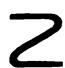
\includegraphics[keepaspectratio]{images/part002_88480e13.jpg}}

Example. --- A pure basis is a transcendence basis. On the other hand, if E is a pure extension of K, a transcendence basis of E over K is not always a pure basis of E. For example, in \(\mathbf{K}(\mathbf{X})\) , \(\{\mathbf{X}^{2}\}\) is a transcendence basis but does not generate \(\mathbf{K}(\mathbf{X})\) .

PROPOSITION 7. --- Let E be an extension of a field K. Every transcendence basis of E is a maximal element of the set (ordered by inclusion) of subsets of E algebraically free over K. Conversely, if S is a subset of E such that E is algebraic over K(S), every maximal algebraically free subset of S is a transcendence basis of E.

Let B be a transcendence basis of E over K and \(x \in E - B\) . Then x is algebraic over \(\mathrm{K}(\mathrm{B})\) ; by V, p.~107, Prop. 4, the subset \(B \cup \{x\}\) of E is not algebraically free over K, whence the first part of the proposition. Secondly, if E is algebraic over \(\mathrm{K}(\mathrm{S})\) and B is a maximal algebraically free part of S, it follows from the Cor. of Prop. 4 that every \(x \in S\) is algebraic over \(\mathrm{K}(\mathrm{B})\) ; hence (V, p.~18, Cor. 1) \(\mathrm{K}(\mathrm{S})\) is algebraic over \(\mathrm{K}(\mathrm{B})\) , and so (V, p.~19, Prop. 3), E is algebraic over \(\mathrm{K}(\mathrm{B})\) .

THEOREM 1 (Steinitz). --- Every extension E of a field K admits a transcendence basis over K. In other words, every extension of a field K is an algebraic extension of a pure extension of K.

\pandocbounded{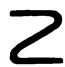
\includegraphics[keepaspectratio]{images/part002_71d10db7.jpg}}

By contrast, an extension is not always a pure extension of an algebraic extension (V, p.~171, Ex. 2).

This theorem is a consequence of the following more precise result:

THEOREM 2. --- Let E be an extension of a field K, S a subset of E such that E is algebraic over K(S) and T a subset of S which is algebraically free over K; then there exists a transcendence basis B of E over K such that \(T \subset B \subset S\) .

For the set of algebraically free subsets of S, ordered by inclusion, is a set of finite character (E, III, p.~34) by Prop. 3. By Th. 1 of E, III, p.~35 it has a maximal element B containing T, and B is a transcendence basis of E over K, by Prop. 7.

COROLLARY (« Exchange Theorem »). --- Let E be an extension of K, S a subset of E such that E is algebraic over K(S), T a subset of E which is algebraically free over K; then there exists a subset S' of S such that T ∪ S' is a transcendence basis of E over K and T ∩ S' = ∅.

For E is algebraic over \(\mathbf{K}(\mathbf{T} \cup \mathbf{S})\) and we have \(T \subset T \cup S\) .

\subsection{The transcendence degree of an extension}

THEOREM 3. --- Let E be an extension of a field K. All transcendence bases of E over K have the same cardinal.

It is enough to prove the inequality \(\operatorname{Card}(\mathbf{B}) \geqslant \operatorname{Card}(\mathbf{B}')\) , when \(\mathbf{B}\) and \(\mathbf{B}'\) are two transcendence bases of \(\mathbf{E}\) over \(\mathbf{K}\) , and we may suppose that \(\mathbf{B}'\) is not empty. We first suppose that \(\mathbf{B}\) is finite and use induction on its cardinal \(n\) ; for \(n = 0\) , \(\mathbf{E}\) is algebraic over \(\mathbf{K}\) and \(\mathbf{B}'\) is empty. Suppose now that \(n \geqslant 1\) ; given \(x \in \mathbf{B}'\) , the exchange theorem provides a subset \(\mathbf{C}\) of \(\mathbf{B}\) such that \(x \notin \mathbf{C}\) and \(\{x\} \cup \mathbf{C}\) is a transcendence basis of \(\mathbf{E}\) over \(\mathbf{K}\) ; we have \(\mathbf{C} \neq \mathbf{B}\) by Prop. 7 whence \(\operatorname{Card} \mathbf{C} < n\) . Put \(\mathbf{K}_1 = \mathbf{K}(x)\) and \(\mathbf{C}' = \mathbf{B}' - \{x\}\) ; then \(\mathbf{C}\) and \(\mathbf{C}'\) are algebraically free over the field \(\mathbf{K}_1\) (V, p.~107, Prop. 4) and \(\mathbf{E}\) is algebraic both over \(\mathbf{K}_1(\mathbf{C}) = \mathbf{K}(\mathbf{C} \cup \{x\})\) and \(\mathbf{K}_1(\mathbf{C}') = \mathbf{K}(\mathbf{B}')\) . In other words, \(\mathbf{C}\) and \(\mathbf{C}'\) are two transcendence bases of \(\mathbf{E}\) over \(\mathbf{K}_1\) . Since \(\operatorname{Card}(\mathbf{C}) < n\) , the induction hypothesis implies the inequality \(\operatorname{Card}(\mathbf{C}') \leqslant \operatorname{Card}(\mathbf{C}) \leqslant n - 1\) , whence \(\operatorname{Card}(\mathbf{B}') \leqslant n = \operatorname{Card}(\mathbf{B})\) .

Suppose now that B is infinite. Every \(x \in B\) is algebraic over \(\mathrm{K}(\mathrm{B}')\) and so there exists a finite subset \(\mathrm{S}(x)\) of \(B'\) such that x is algebraic over \(\mathrm{K}(\mathrm{S}(x))\) . Write \(\mathrm{S} = \bigcup_{x \in \mathrm{B}} \mathrm{S}(x)\) , then \(S \subset B'\) and since B is infinite, we have \(\operatorname{Card}(\mathrm{S}) \leqslant \operatorname{Card}(\mathrm{B})\)

(E, III, p.~49, Cor. 3). But since every element of B is algebraic over K(S) and E is algebraic over K(B), we conclude that E is algebraic over K(S) (V, p.~19, Prop. 3). Now Prop. 7 implies that S = B', whence the desired inequality Card(B') ≤ Card(B).

DEFINITION 4. --- Let E be an extension of a field K. The cardinal of every transcendence basis of E over K is called the transcendence degree of E over K and written tr. deg \(_{K}\) E.

Th. 2 and 3 and Def. 4 imply the following corollaries, where E denotes an extension of a field K, of finite transcendence degree n.

COROLLARY 1. --- Let S be a subset of E such that E is algebraic over K(S). Then Card(S) ≥ n ; if the cardinal of S is equal to n, then S is algebraically free over K (hence it is then a transcendence basis of E over K).

COROLLARY 2. --- Suppose that \(\mathrm{E} = \mathrm{K}(x_1, \ldots, x_m)\) , then \(m \geqslant n\) ; if moreover \(m = n\) , then \((x_1, \ldots, x_m)\) is a pure basis of \(\mathrm{E}\) over \(\mathrm{K}\) , and \(\mathrm{E}\) is then a pure extension of \(\mathrm{K}\) .

COROLLARY 3. --- Every subset of E which is algebraically free over K has at most n elements, and if it has exactly n elements, it is a transcendence basis of E over K.

THEOREM 4. --- Let K, E and F be three fields such that \(K \subset E \subset F\) . If S is a transcendence basis of E over K and T a transcendence basis of F over E, then \(S \cap T\) is empty and \(S \cup T\) is a transcendence basis of F over K.

For F is algebraic over \(E(T)\) ; moreover, \(E(T)\) is algebraic over the field \(K(S \cup T) = K(S)(T)\) , because E is algebraic over \(K(S)\) (V, p.~18, Cor. 2); therefore (V, p.~19, Prop. 3) F is algebraic over \(K(S \cup T)\) . On the other hand, T being algebraically free over E is so a fortiori over \(K(S)\) , hence (V, p.~107, Prop. 4) \(S \cup T\) is algebraically free over K and \(S \cap T = \varnothing\) .

COROLLARY. --- Let K, E and F be three fields such that \(K \subset E \subset F\) . Then we have

\[
\operatorname{tr} \cdot \deg_ {K} F = \operatorname{tr} \cdot \deg_ {K} E + \operatorname{tr} \cdot \deg_ {E} F.\tag{1}
\]

\subsection{Extension of isomorphisms}

PROPOSITION 8. --- Let \(\Omega\) be an algebraically closed extension of a field K, E and F two subextensions of \(\Omega\) and \(u\) a K-isomorphism of E onto F. For a K-automorphism \(v\) of \(\Omega\) to exist which extends \(u\) , it is necessary and sufficient for \(\Omega\) to have the same transcendence degree over E and F.

The condition is clearly necessary.

Suppose then that \(\Omega\) has the same transcendence degree over E and F and let us choose a transcendence basis B of \(\Omega\) over E and a transcendence basis C of \(\Omega\) over F. Since B and C are equipotent, Prop. 2 (V, p.~106) shows that \(u\) extends to a K-isomorphism \(u'\) of E(B) onto F(C). Since \(\Omega\) is an algebraic closure of E(B) and F(C), the Cor. of V, p.~23 shows that \(u'\) extends to an automorphism \(v\) of \(\Omega\) .

COROLLARY 1. --- Let \(\Omega\) be an algebraically closed extension of a field K and E a subextension of \(\Omega\) . Every K-automorphism of E extends to a K-automorphism of \(\Omega\) .

COROLLARY 2. --- Let \(\Omega\) be an algebraically closed extension of a field \(K\) , \(E\) and \(F\) two subextensions of \(\Omega\) and \(u\) a K-isomorphism of \(E\) onto \(F\) . If the transcendence degree of \(E\) over \(K\) is finite (in particular if \(E\) is algebraic over \(K\) ) then there exists a K-automorphism of \(\Omega\) extending \(u\) .

Let us denote by n, \(d(\mathrm{E})\) and \(d(\mathrm{F})\) the transcendence degrees of E over K, of \(\Omega\) over E and of \(\Omega\) over F respectively. The existence of the K-isomorphism u shows that the transcendence degree of F over K is equal to n.~By the Cor. of Th. 4 the transcendence degree of \(\Omega\) over K is equal to \(d(\mathrm{E}) + n\) and also to \(d(\mathrm{F}) + n\) . Therefore (E, III, p.~28, Prop. 8) we have \(d(\mathrm{E}) = d(\mathrm{F})\) and we can apply Prop. 8.

PROPOSITION 9. --- Let K be a field and \(\Omega\) an algebraically closed extension of K. Suppose that \(\Omega\) is not algebraic over K; then the set of elements of \(\Omega\) which are transcendental over K is infinite. Moreover, if \(x\) and \(y\) are two elements of \(\Omega\) which are transcendental over K, then there exists an automorphism \(u\) of \(\Omega\) over K such that \(u(x) = y\) .

Since \(\Omega\) is not algebraic over \(\mathbf{K}\) , there exists an element \(x\) of \(\Omega\) transcendental over \(\mathbf{K}\) ; then the elements \(x^n\) ( \(n \in \mathbf{N}\) ) are distinct and transcendental over \(\mathbf{K}\) . Suppose that \(x\) and \(y\) are distinct and transcendental over \(\mathbf{K}\) ; by Prop. 2 (V, p.~106) there exists a K-isomorphism \(\tilde{u}\) of \(\mathbf{K}(x)\) onto \(\mathbf{K}(y)\) such that \(\tilde{u}(x) = y\) ; since \(\mathbf{K}(x)\) is of transcendence degree 1 over \(\mathbf{K}\) , Cor. 2 of Prop. 8 shows that \(\tilde{u}\) extends to a K-automorphism \(u\) of \(\Omega\) .

PROPOSITION 10. --- Let K be a field, Ω an algebraically closed extension of K and G the group of K-automorphisms of Ω. Let \(x \in \Omega\) .

\begin{enumerate}
\def\labelenumi{\alph{enumi})}
\item
  For \(x\) to be algebraic over \(K\) it is necessary and sufficient for the set of elements \(u(x)\) as \(u\) runs over \(G\) to be finite,
\item
  For \(x\) to be \(p\) -radical over \(\mathbf{K}\) it is necessary and sufficient that \(u(x) = x\) for all \(u \in \mathbf{G}\) .
\end{enumerate}

In particular if K is perfect, the set of invariants of the group G is equal to K. Suppose first that x is transcendental. By Prop. 9 the set T of elements of \(\Omega\) transcendental over K is infinite, and for each \(y \in T\) there exists \(u \in G\) such that \(u(x) = y\) . Hence the set of elements \(u(x)\) as u runs over G is infinite.

Suppose now that \(x\) is algebraic over \(\mathbf{K}\) and denote by \(f\) its minimal polynomial over \(\mathbf{K}\) ; the set of roots of \(f\) in \(\Omega\) is finite and for each \(u \in \mathbf{G}\) we have \(f(u(x)) = u(f(x)) = 0\) . Hence the set of elements \(u(x)\) as \(u\) runs over \(\mathbf{G}\) is finite. This proves \(a\) .

Let L be the set of elements y of \(\Omega\) such that \(u(y)=y\) for all \(u\in G\) , and let \(\bar{K}\) be the relative algebraic closure of K in \(\Omega\) . By what has been said, L is a subextension of \(\bar{K}\) over K. Further (Cor. 1 to Prop. 8) every K-automorphism of \(\bar{K}\) is the restriction to \(\bar{K}\) of an element of G. Assertion b) of Prop. 10 now follows from Cor. 3 of V, p.~53.

\subsection{Algebraically disjoint extensions}

DEFINITION 5. --- Let L be an extension of a field K, and E and F two subextensions of L. Then E and F are said to be algebraically disjoint (over K) and E is said to be algebraically disjoint from F over K, if for every subset A (resp. B) of E (resp. F) algebraically free over K, A and B are disjoint and A ∪ B is algebraically free over K.

Remarks. --- 1) If E is a subextension of L which is algebraic over K, then it is algebraically disjoint from every subextension F of L. For an extension of K to be algebraic it is necessary and sufficient that it should be algebraically disjoint from itself.

\begin{enumerate}
\def\labelenumi{\arabic{enumi})}
\setcounter{enumi}{1}
\item
  It may happen that E is algebraically disjoint from F over K, but not over a subfield \(K_{0}\) of K. * For example C is algebraically disjoint from itself over R but not over Q. *
\item
  It is clear that if E is algebraically disjoint from F over K, when E and F are considered as subextensions of L, the same is true when they are considered as subextensions of \(\mathbf{K}(\mathbf{E} \cup \mathbf{F})\) and conversely.
\end{enumerate}

PROPOSITION 11. --- If E and F are algebraically disjoint over K then E ∩ F is algebraic over K.

This follows from Def. 5.

PROPOSITION 12. --- Let L be an extension of a field K and E, F subextensions of L. Then the following conditions are equivalent :

\begin{enumerate}
\def\labelenumi{\alph{enumi})}
\item
  E and F are algebraically disjoint;
\item
  there exists a transcendence basis of E over K which is algebraically free over F;
\item
  every subset of E which is algebraically free over K is algebraically free over F. Let us introduce the following conditions:
\end{enumerate}

\(b^{\prime})\) there exists a transcendence basis of \(\mathbf{F}\) over \(\mathbf{K}\) which is algebraically free over \(\mathbf{E}\) ;

\(c^{\prime})\) every subset of \(\mathbf{F}\) which is algebraically free over \(\mathbf{K}\) is algebraically free over \(\mathbf{E}\) .

\(a) \Rightarrow b')\) : Suppose that E and F are algebraically disjoint. Let B (resp. C) be a transcendence basis of E (resp. F) over K. Then \(B \cap C = \emptyset\) and \(B \cup C\) is algebraically free over K, hence C is algebraically free over \(K(B)\) (V, p.~107, Prop. 4); since E is algebraic over \(K(B)\) , Prop. 6 of V, p.~108 shows C to be algebraically free over E.

\(b') \Rightarrow c)\) : Suppose that there exists a transcendence basis C of F over K which is algebraically free over E. Let A be a subset of E algebraically free over K. Then C is algebraically free over K(A), hence A is algebraically free over K(C) (V, p.~107, Prop. 4) and therefore over F (V, p.~108, Prop. 6), because F is algebraic over K(C).

\(c) \Rightarrow a)\) : This follows at once from Prop. 4 (V, p.~107).

The implications \(a) \Rightarrow b) \Rightarrow c') \Rightarrow a)\) may be proved in the same way.

COROLLARY. --- Let E and F be algebraically disjoint over K. Let E' be the relative algebraic closure of E in L and F' that of F (V, p.~19). Then E' and F' are algebraically disjoint over K.

Let B be a transcendence basis of E over K; this is also a transcendence basis of \(E'\) over K. Since E is algebraically disjoint from F over K, B is algebraically free over F, hence over \(F'\) (V, p.~108, Prop. 6); now we can apply Prop. 12.

PROPOSITION 13. --- Let L be an extension of a field K and E, F two subextensions of L.

\begin{enumerate}
\def\labelenumi{\alph{enumi})}
\tightlist
\item
  We have \(\operatorname{tr} \cdot \deg_{\mathbb{F}} \mathrm{F}(\mathrm{E}) \leqslant \operatorname{tr} \cdot \deg_{\mathbb{K}} \mathrm{E}\) . When \(\mathrm{E}\) and \(\mathrm{F}\) are algebraically disjoint over \(\mathbf{K}\) , then every transcendence basis of \(\mathrm{E}\) over \(\mathbf{K}\) is a transcendence basis of
\end{enumerate}

\(F(E)\) over F and we have tr. \(\deg_{F}F(E) = \text{tr. } \deg_{K}E\) . Conversely, this equality implies that E and F are algebraically disjoint over K when tr. \(\deg_{K}E\) is finite.

\begin{enumerate}
\def\labelenumi{\alph{enumi})}
\setcounter{enumi}{1}
\item
  We have \(\operatorname{tr} \cdot \deg_{\mathbf{K}} \mathrm{K}(\mathrm{E} \cup \mathrm{F}) \leqslant \operatorname{tr} \cdot \deg_{\mathbf{K}} \mathrm{E} + \operatorname{tr} \cdot \deg_{\mathbf{K}} \mathrm{F}\) . When \(\mathrm{E}\) and \(\mathrm{F}\) are algebraically disjoint over \(\mathbf{K}\) , we have \(\operatorname{tr} \cdot \deg_{\mathbf{K}} \mathrm{K}(\mathrm{E} \cup \mathrm{F}) = \operatorname{tr} \cdot \deg_{\mathbf{K}} \mathrm{E} + \operatorname{tr} \cdot \deg_{\mathbf{K}} \mathrm{F}\) . Conversely, this equality implies that \(\mathrm{E}\) and \(\mathrm{F}\) are algebraically disjoint over \(\mathbf{K}\) when \(\mathrm{E}\) and \(\mathrm{F}\) are of finite transcendence degree over \(\mathbf{K}\) .
\item
  Let B be a transcendence basis of E over K; then E is algebraic over K(B), and Cor. 2 of V, p.~18 shows that F(E) is algebraic over F(K(B)) = F(B). By Th. 2 (V, p.~109) B contains a transcendence basis of F(E) over F; when E is algebraically disjoint from F over K, B is algebraically free over F (Prop. 12) and this is then a transcendence basis of F(E) over F. The three first assertions of a) follow from this. Suppose now that E is of finite transcendence degree over K, equal to that of F(E) over F; since F(E) is algebraic over F(B) and Card B = tr . deg\_F F(E), Cor. 1 of V, p.~110 shows B to be algebraically free over F, so E is algebraically disjoint from F over K (Prop. 12).
\item
  We have \(\mathbf{K}(\mathbf{E} \cup \mathbf{F}) = \mathbf{F}(\mathbf{E})\) and so the Cor. of V, p.~110 implies the equality:
\end{enumerate}

\[
\operatorname{tr} \cdot \deg_ {K} K (E \cup F) = \operatorname{tr} \cdot \deg_ {F} F (E) + \operatorname{tr} \cdot \deg_ {K} F.
\]

Now \(b)\) follows at once from \(a)\) and this equality.

PROPOSITION 14. --- Let L be an extension of a field K, E and F two subextensions of L and B a transcendence basis of E over K. For E and F to be algebraically disjoint over K it is necessary and sufficient that K(B) and F should be linearly disjoint over K.

For E and F to be algebraically disjoint over K it is necessary and sufficient for B to be algebraically free over F (Prop. 12), that is, for the monomials in the elements of B to be linearly independent over F. Since these monomials form a basis of the vector K-space K{[}B{]}, it comes to the same to say that K{[}B{]} and F are linearly disjoint over K. Finally, since K(B) is the field of fractions of K{[}B{]}, Prop. 6 of V, p.~14 shows that K{[}B{]} and F are linearly disjoint if and only if this is so for K(B) and F.

COROLLARY 1. --- If E and F are linearly disjoint, then E is algebraically disjoint from F over K. Conversely, if E is a pure extension of K and is algebraically disjoint from F over K, then E and F are linearly disjoint over K.

COROLLARY 2. --- Every pure extension of K is linearly disjoint from every algebraic extension of K; in particular, K is relatively algebraically closed in every pure extension of K.

\subsection{Algebraically free families of extensions}

DEFINITION 6. --- Let L be an extension of a field K and \((\mathrm{E}_{i})_{i\in I}\) a family of subextensions of L. The family \((\mathrm{E}_{i})_{i\in I}\) is said to be algebraically free if the following condition is satisfied:

(AF) For each \(i \in I\) let \(\mathbf{A}_i\) be a subset of \(\mathbf{E}_i\) which is algebraically free over \(\mathbf{K}\) . Then \(\mathbf{A}_i \cap \mathbf{A}_j = \emptyset\) for \(i \neq j\) and \(\cup \mathbf{A}_i\) is algebraically free over \(\mathbf{K}\) .

Remark. --- By Prop. 3 (V, p.~107) it is enough to verify the condition (AF) for finite subsets \(A_{i}\) . We thus obtain the following result: if \((\mathrm{E}_{i})_{i\in I}\) is an algebraically free family, the same is true of \((\mathrm{E}_{i}^{\prime})_{i\in I}\) if \(E_{i}^{\prime}\) is a subextension of \(E_{i}\) for each \(i\in I\) ; conversely, if every family \((\mathrm{E}_{i}^{\prime})_{i\in I}\) , where \(E_{i}^{\prime}\) is a finitely generated subextension of E for each \(i\in I\) is algebraically free, then \((\mathrm{E}_{i})_{i\in I}\) is algebraically free. On the other hand, for \((\mathrm{E}_{i})_{i\in I}\) to be algebraically free it is necessary and sufficient that \((\mathrm{E}_{i})_{i\in J}\) should be algebraically free for every finite subset J of I. Speaking intuitively we may say that the algebraic independence of extensions is a property « of finite character ».

PROPOSITION 15. --- Let \((\mathbf{E}_i)_{i\in I}\) be a family of subextensions of a given extension L of a field K. Then the following conditions are equivalent:

\begin{enumerate}
\def\labelenumi{\alph{enumi})}
\item
  The family \((\mathrm{E}_i)_{i\in I}\) is algebraically free.
\item
  For each \(i \in I\) the extension \(E_i\) is algebraically disjoint over \(K\) from the extension \(F_i\) generated by the \(E_j\) for \(j \neq i\) .
\item
  There exists a family \((\mathbf{B}_i)_{i\in I}\) of disjoint subsets of \(L\) , such that \(\mathbf{B}_i\) is a transcendence basis of \(\mathbf{E}_i\) over \(K\) for each \(i\in I\) , and \(\mathbf{B} = \bigcup_{i\in I}\mathbf{B}_i\) is algebraically free over \(K\) .
\end{enumerate}

It is clear that \(a)\) implies \(c)\) .

Assuming \(c\) ), let us choose \(i\) in \(I\) ; put \(C_i = \bigcup_{j \neq i} B_j\) . For each \(j \neq i\) every element

of \(E_{j}\) is algebraic over \(\mathbf{K}(\mathbf{B}_{j})\) and a fortiori over \(\mathbf{K}(\mathbf{C}_{i})\) . By Cor. 1 of V, p.~18, the field \(F_{i}\) is therefore algebraic over \(\mathbf{K}(\mathbf{C}_{i})\) . Further, we have \(B_{i} \cap C_{i} = \varnothing\) and \(B = B_{i} \cup C_{i}\) is algebraically free over K; therefore \(B_{i}\) is algebraically free over \(\mathbf{K}(\mathbf{C}_{i})\) (V, p.~107, Prop. 4), hence also over \(F_{i}\) (which is algebraic over \(\mathbf{K}(\mathbf{C}_{i})\) ) by Prop. 6 of V, p.~108. Thus we have proved that \(E_{i}\) is algebraically disjoint from \(F_{i}\) over K (V, p.~113, Prop. 12), hence c) implies b).

Let us now assume \(b)\) and prove \(a)\) . It is enough to show that if \(i_1, \ldots, i_n\) are distinct elements of \(I\) , then the family of extensions \((E_{i_1}, \ldots, E_{i_n})\) is algebraically free; we argue by induction on \(n\) , the case \(n = 1\) being trivial. Suppose then that \(n > 1\) and that the family \((E_{i_1}, \ldots, E_{i_{n-1}})\) is algebraically free; for \(1 \leqslant k \leqslant n\) choose a subset \(A_k\) of \(E_{i_k}\) algebraically free over \(K\) and put

\(B = A_{1} \cup \ldots \cup A_{n-1}\) . By the induction hypothesis the subsets \(A_{1}, \ldots, A_{n-1}\) are pairwise disjoint and B is algebraically free over K; by b) \(E_{i_{n}}\) is algebraically disjoint from \(F_{i_{n}}\) and since B is contained in \(F_{i_{n}}\) we have \(B \cap A_{n} = \varnothing\) and \(B \cup A_{n} = A_{1} \cup \ldots \cup A_{n}\) is algebraically free over K. We have thus shown that the family \((E_{i_{1}}, \ldots, E_{i_{n}})\) is algebraically free.

The following proposition generalizes part \(b)\) of Prop. 13 (V, p.~113).

PROPOSITION 16. --- Let \((\mathrm{E}_i)_{i\in I}\) be a family of subextensions of an extension of a field K, and let E be the field generated by \(\cup\) \(\mathrm{E}_i\) .

\begin{enumerate}
\def\labelenumi{\alph{enumi})}
\item
  We have \(\operatorname{tr} \cdot \deg_{\mathbf{K}} \mathrm{E} \leqslant \sum_{i \in I} \operatorname{tr} \cdot \deg_{\mathbf{K}} \mathrm{E}_i\) , with equality when the family \((\mathrm{E}_i)_{i \in I}\) is algebraically free over \(\mathbf{K}\) .
\item
  Conversely, assume that \(\operatorname{tr} \cdot \deg_{\mathbf{K}} \mathrm{E} = \sum_{i \in I} \operatorname{tr} \cdot \deg_{\mathbf{K}} \mathrm{E}_i\) and that \(\operatorname{tr} \cdot \deg_{\mathbf{K}} \mathrm{E}\) is finite; then the family \((\mathrm{E}_i)_{i \in I}\) is algebraically free over \(\mathbf{K}\) .
\end{enumerate}

For each \(i \in I\) let \(\mathbf{B}_i\) be a transcendence basis of \(\mathbf{E}_i\) over \(\mathbf{K}\) and put \(\mathbf{B} = \bigcup_{i \in I} \mathbf{B}_i\) . For each \(i \in I\) , each element of \(\mathbf{E}_i\) is algebraic over \(\mathbf{K}(\mathbf{B}_i)\) , hence over

K(B). Now Cor. 1 of V, p.~18 shows that E is algebraic over K(B); by V, p.~109, Th. 2, B thus contains a transcendence basis of E over K. If moreover the family \((\mathrm{E}_{i})_{i\in I}\) is algebraically free over K, then the \(B_{i}\) are disjoint and the set B is algebraically free over K. This establishes a) (Set Theory, III, p.~160, Cor. of Prop. 4).

Under the hypotheses of \(b\) ), E is algebraic over \(\mathbf{K}(\mathbf{B})\) and of finite transcendence degree over \(\mathbf{K}\) , and we have \(\operatorname{Card}(\mathbf{B}) \leqslant \operatorname{tr} \cdot \deg_{\mathbf{K}} \operatorname{E}\) . By Cor. 1 of V, p.~110, B is algebraically free over \(\mathbf{K}\) and the \(\mathbf{B}_i\) are disjoint. Now Prop. 15 shows that the family \((\mathrm{E}_i)_{i \in I}\) is algebraically free over \(\mathbf{K}\) .

Before stating the next theorem let us remark that there exist algebraically closed extensions of K of arbitrary transcendence degree, for example an algebraic closure of an appropriate field of rational fractions.

THEOREM 5. --- Let \((\mathrm{E}_i)_{i\in I}\) be a family of extensions of a field \(\mathbf{K}\) and \(\Omega\) an algebraically closed extension of \(\mathbf{K}\) . Suppose that the inequality

\[
\operatorname{tr} \cdot \deg_ {K} \Omega \geqslant \sum_ {i \in I} \operatorname{tr} \cdot \deg_ {K} E _ {i}\tag{2}
\]

holds. Then there exists an algebraically free family \((\mathrm{F}_i)_{i\in I}\) of subextensions of \(\Omega\) such that \(\mathbf{F}_i\) is K-isomorphic to \(\mathbf{E}_i\) for all \(i\in I\) .

For each \(i \in I\) let \(B_i\) be a transcendence basis of \(E_i\) over \(K\) . Let \(B\) be a transcendence basis of \(\Omega\) over \(K\) . By (2) we have Card \(B \geqslant \sum_{i \in I} \text{Card } B_i\) ; hence

there exists a family \((\mathbf{B}_{i}^{\prime})_{i\in I}\) of pairwise disjoint subsets of B and bijections \(u_{i}:B_{i}\to B_{i}^{\prime}\) (for \(i\in I\) ). By Prop. 2 of V, p.~106, \(u_{i}\) extends to a K-isomorphism \(v_{i}\) of \(\mathbf{K}(\mathbf{B}_{i})\) onto \(\mathbf{K}(\mathbf{B}_{i}^{\prime})\) ; since \(\Omega\) is algebraically closed and \(E_{i}\) algebraic over

\(K(B_{i})\) , the Cor. (V, p.~23) shows that \(v_{i}\) extends to a K-isomorphism of \(E_{i}\) onto a subextension \(F_{i}\) of \(\Omega\) . By construction \(B_{i}^{\prime}\) is a transcendence basis of \(F_{i}\) over K, and Prop. 15 (V, p.~115) shows that the family \((F_{i})_{i\in I}\) of subextensions of \(\Omega\) is algebraically free over K.

COROLLARY 1. --- Let E and Ω be two extensions of a field K. Suppose that Ω is algebraically closed, of transcendence degree at least equal to that of E. Then E is K-isomorphic to a subextension of Ω.

COROLLARY 2. --- Let \(\Omega\) be an algebraically closed field of infinite transcendence degree over its prime subfield. Then every field of the same characteristic as \(\Omega\) is the ascending directed union of fields isomorphic to subfields of \(\Omega\) .

For each field is the ascending directed union of finitely generated subfields over its prime field, and now it is enough to apply Cor. 1.

* Example. --- This applies particularly in characteristic 0 in taking \(\Omega = \mathbf{C}\) (« Lefschetz' principle »). *

\subsection{Finitely generated extensions}

PROPOSITION 17. --- Let E be an extension of a field K and B a transcendence basis of E over K. For E to be finitely generated over K (V, p.~11, Def. 2) it is necessary and sufficient that B be finite and that the degree {[}E : K(B){]} be finite.

Suppose that E is finitely generated over K and let S be a finite subset of E such that \(\mathrm{E} = \mathrm{K}(\mathrm{S})\) . By Th. 2 (V, p.~109) S contains a transcendence basis \(B'\) of E over K and this has the same cardinal as B (V, p.~110, Th. 3). Therefore B is finite. Put \(\mathrm{K}' = \mathrm{K}(\mathrm{B})\) ; then E is algebraic over \(K'\) and we have \(\mathrm{E} = \mathrm{K}'(\mathrm{S})\) ; since S is finite, Th. 2 of V, p.~18 shows that \([E : K']\) is finite.

Conversely, suppose that B is finite and \([E:K(B)]\) is finite. If C is a (finite) basis of the vector space E over \(K(B)\) , we have \(E = K(B)(C) = K(B \cup C)\) and so E is a finitely generated extension of K.

COROLLARY 1. --- Suppose that E is a finitely generated extension of K, and let K' be the relative algebraic closure of K in E (V, p.~19). Then K' is of finite degree over K.

Let B be a transcendence basis of E over K. By Cor. 2 of V, p.~114, \(K'\) is linearly disjoint from \(\mathrm{K}(\mathrm{B})\) over K, whence \([\mathrm{K}' : \mathrm{K}] = [\mathrm{K}'(\mathrm{B}) : \mathrm{K}(\mathrm{B})] \leq [\mathrm{E} : \mathrm{K}(\mathrm{B})]\) and now the finiteness of \([\mathrm{K}' : \mathrm{K}]\) follows from that of \([\mathrm{E} : \mathrm{K}(\mathrm{B})]\) .

COROLLARY 2. --- A field that is finitely generated over its prime subfield contains only finitely many roots of unity.

By Cor. 1 we are reduced to proving that a field L which is an extension of finite degree of its prime subfield possesses only a finite number of roots of unity. This is clear when L is of characteristic \(\neq0\) because it is then finite. If L is of characteristic 0 and contains infinitely many roots of unity, then it contains primitive roots of unity of arbitrarily high order. By V, p.~84, Th. 2 there exist therefore an infinity of integers n \textgreater{} 0 such that \(\varphi(n) \leqslant [L : Q]\) , which is absurd (V, p.~80, Formulae (2) and (3)).

COROLLARY 3. --- If E is a finitely generated extension of a field K, then every subextension E' of E is finitely generated.

Let \(B'\) be a transcendence basis of \(E'\) over \(K\) . By \(V\) , p.~109, Th. 2, \(B'\) is contained in a transcendence basis \(B\) of \(E\) over \(K\) and so is finite, by Prop. 17. Since \(E'\) is algebraic over \(K(B')\) and \(E\) is a finitely generated extension of \(K(B')\) , Cor. 1 shows \([E': K(B')]\) to be finite. Now Prop. 17 shows that \(E'\) is finitely generated over \(K\) .

Prop. 17 may be paraphrased by saying that a finitely generated extension of K is an algebraic extension of finite degree of a purely transcendental extension \(\mathrm{K}(x_{1},\ldots,x_{n})\) .

\section{SEPARABLE EXTENSIONS}

\subsection{Characterization of the nilpotent elements of a ring}

PROPOSITION 1. --- Let A be a commutative ring and x an element of A. For x to be nilpotent it is necessary and sufficient that 1 - xT be invertible in the ring A{[}T{]}.

We note that A{[}T{]} is a subring of the formal power series ring A{[}{[}T{]}{]} and that 1 - xT has in A{[}{[}T{]}{]} the inverse \(\sum_{n=0}^{\infty} x^{n} T^{n}\) (IV, p.~30, Prop. 5). For 1 - xT to be

invertible in A{[}T{]} it is necessary and sufficient for \(\sum_{n=0}^{\infty} x^n T^n\) to be a polynomial,

that is, for \(x\) to be nilpotent.

PROPOSITION 2. --- Let A be a commutative ring. The set of nilpotent elements of A is an ideal of A equal to the intersection of the set of all prime ideals of A.

Let \(x\) be a nilpotent element of \(\mathbf{A}\) and \(\mathfrak{p}\) a prime ideal of \(\mathbf{A}\) . The residue class of \(x \mod \mathfrak{p}\) is a nilpotent element of the integral domain \(\mathbf{A} / \mathfrak{p}\) , hence is zero; thus we have \(x \in \mathfrak{p}\) .

Let \(x\) be a non-nilpotent element of \(A\) . By Prop. 1 the principal ideal \((1 - xT)\) of \(A[T]\) is distinct from \(A[T]\) . By Krull's theorem (I, p.~104) there exists a maximal ideal \(m\) of \(A[T]\) containing \(1 - xT\) . Then \(m\) is a prime ideal of \(A[T]\) , hence \(p = A \cap m\) is a prime ideal of \(A\) . We have \(1 \notin m\) and \(1 - Tx \in m\) , hence \(Tx \notin m\) and a fortiori \(x \notin p\) .

We have thus shown that the set n of nilpotent elements of A is the intersection of the set of all prime ideals of A; since every intersection of ideals is an ideal, n is an ideal.

COROLLARY. --- For a commutative ring to be reduced (V, p.~34, Def. 2) it is necessary and sufficient for it to be isomorphic to a subring of a product of fields.

The condition is clearly sufficient.

Let A be reduced. By Prop. 2 the intersection n of the set of prime ideals of A is reduced to 0. For every prime ideal p of A, let \(k(\mathfrak{p})\) be the field of fractions of A/p and \(\varphi_{p}\) the canonical homomorphism of A into \(k(\mathfrak{p})\) . Let \(\varphi\) be the homomorphism of A into \(\prod_{\mathfrak{p}} k(\mathfrak{p})\) whose component of index p is \(\varphi_{p}\) . The kernel of \(\varphi_{\mathfrak{p}}\) is \(\mathfrak{p}\) , hence that of \(\varphi\) is \(\mathfrak{n} = 0\) ; therefore \(\varphi\) is an isomorphism of \(\mathbf{A}\) onto a subring of \(\prod_{\mathfrak{p}} k(\mathfrak{p})\) .

\subsection{Separable algebras}

DEFINITION 1. --- Let A be a commutative algebra over a field K. Then A is said to be separable over K, or also a separable K-algebra if the ring L ⊗K A is reduced for every extension L of K.

Every separable algebra is clearly reduced. For a partial converse see Th. 3 (V, p.~125).

Examples. --- 1) Let A be a polynomial algebra \(K[X_{i}]_{i \in I}\) . For every extension L of K the ring \(L \otimes_{K} A\) is isomorphic to \(L[X_{i}]_{i \in I}\) (III, p.~449, Remark 2) and hence is an integral domain (IV, p.~9, Prop. 8). In other words, every polynomial algebra over a field K is a separable K-algebra.

\begin{enumerate}
\def\labelenumi{\arabic{enumi})}
\setcounter{enumi}{1}
\item
  Let A be a commutative algebra of finite degree over a field K. For A to be separable it is necessary and sufficient for it to be etale (V, p.~34, Th. 4).
\item
  Let E be an algebraic extension of a field K. If L is an extension of K, then the ring \(L \otimes_{K} E\) is a union of the subrings \(L \otimes_{K} F\) where F ranges over the set of all subextensions of finite degree of E; therefore the ring \(L \otimes_{K} E\) is reduced if and only if this is true of \(L \otimes_{K} F\) for every subextension F of E, of finite degree over K. Taking Example 2 into account we see that E is a separable algebra in the sense of the above Def. 1 if and only if it is a separable algebraic extension in the sense of Def. 1 of V, p.~36.
\end{enumerate}

PROPOSITION 3. --- Let K be a field.

\begin{enumerate}
\def\labelenumi{\alph{enumi})}
\item
  Every subalgebra of a separable K-algebra is separable.
\item
  Every direct limit of separable K-algebras is separable.
\item
  Every product of separable K-algebras is separable.
\item
  Let A be a K-algebra and \(K'\) an extension of K. For A to be separable it is necessary and sufficient for the \(K'\) -algebra \(\mathbf{A}_{(\mathbf{K}')}\) obtained from A by extension of scalars to be separable.
\end{enumerate}

Let \(\mathbf{L}\) be an extension of \(\mathbf{K}\) . Let \(\mathbf{A}\) be a separable algebra over \(\mathbf{K}\) and \(\mathbf{B}\) a subalgebra of \(\mathbf{A}\) ; then the ring \(\mathbf{L} \otimes_{\mathbf{K}} \mathbf{A}\) is reduced, and \(\mathbf{L} \otimes_{\mathbf{K}} \mathbf{B}\) is isomorphic to a subring of \(\mathbf{L} \otimes_{\mathbf{K}} \mathbf{A}\) , hence is reduced. Thus \(\mathbf{B}\) is separable and \(a)\) is proved. In the same way \(b)\) may be proved, using the canonical isomorphism of \(L \otimes_{K} \varinjlim A_i\) with \(\varinjlim L \otimes_K A_i\) (II, p.~290, Prop. 7) and \(c)\) is proved by remarking that \(L \otimes_K \left( \prod_{i \in I} A_i \right)\) is isomorphic to a subring of \(\prod_{i \in I} (L \otimes_K A_i)\) (II, p.~306, Prop. 15).

We shall use the notation of \(d\) ). For every extension \(\mathbf{L}'\) of \(\mathbf{K}'\) the rings \(\mathbf{L}' \otimes_{\mathbf{K}'} \mathbf{A}_{(\mathbf{K}')}\) and \(\mathbf{L}' \otimes_{\mathbf{K}} \mathbf{A}\) are isomorphic (II, p.~278, Prop. 2). We conclude that if \(\mathbf{A}\) is a separable \(\mathbf{K}\) -algebra, then \(\mathbf{A}_{(\mathbf{K}')}\) is a separable \(\mathbf{K}'\) -algebra. Conversely suppose that \(\mathbf{A}_{(\mathbf{K}')}\) is a separable \(\mathbf{K}'\) -algebra; the preceding remark shows that \(\mathbf{L}' \otimes_{\mathbf{K}} \mathbf{A}\) is reduced for every extension \(\mathbf{L}'\) of \(\mathbf{K}\) containing \(\mathbf{K}'\) as subextension. Let \(\mathbf{L}\) be an extension of \(\mathbf{K}\) ; by the Scholium (V, p.~13) there exists an extension \(\mathbf{L}'\) of \(\mathbf{K}\) containing \(\mathbf{K}'\) as a subextension and a \(\mathbf{K}\) -homomorphism of \(\mathbf{L}\) into \(\mathbf{L}'\) ; the ring \(\mathbf{L} \otimes_{\mathbf{K}} \mathbf{A}\) is thus isomorphic to a subring of \(\mathbf{L}' \otimes_{\mathbf{K}} \mathbf{A}\) and hence reduced. This proves that \(\mathbf{A}\) is a separable \(\mathbf{K}\) -algebra.

PROPOSITION 4. --- Let A be a separable algebra over a field K and let B be the total ring of fractions of A; then the K-algebra B is separable.

Let S be the set of cancellable elements of A. We have identified A with a subring of B (I, p.~113); further, every element of S is invertible in B and every element of B has the form \(as^{-1}\) with \(a \in \mathbf{A}\) and \(s \in \mathbf{S}\) . Let \(L\) be an extension of K and \(x\) a nilpotent element of \(\mathbf{L} \otimes_{\mathbf{K}} \mathbf{B}\) . Then \(x\) may be written in the form \(x = \sum_{i=1}^{n} y_i \otimes a_i s_i^{-1}\) with \(y_i \in \mathbf{L}\) , \(a_i \in \mathbf{A}\) , \(s_i \in \mathbf{S}\) for \(1 \leqslant i \leqslant n\) . If we put \(s = s_1 \ldots s_n\)

then \(x(1 \otimes s)\) belongs to the subring \(L \otimes_{K} A\) of \(L \otimes_{K} B\) ; since \(x(1 \otimes s)\) is nilpotent and A separable over K, we have \(x(1 \otimes s) = 0\) , and since s is invertible in B we find that x = 0. This proves the ring \(L \otimes_{K} B\) to be reduced, whence the proposition.

PROPOSITION 5. --- Let K be a field and A, B commutative K-algebras. If A is reduced and B separable then A ⊗K B is reduced.

By the Cor. of Prop. 2 (V, p.~119) A is isomorphic to a subalgebra of a product \(\prod_{i\in I}L_i\) where \(L_{i}\) is an extension of K for \(i\in I\) . Therefore \(\mathbf{A}\otimes_{\mathbf{K}}\mathbf{B}\) is isomorphic to a

subring of \(\left(\prod_{i\in I}L_i\right)\otimes_K B\) and this latter ring is isomorphic to a subring of

\(\prod_{i\in I}(\mathbf{L}_i\otimes_{\mathbb{K}}\mathbf{B})\) (II, p.~306, Prop. 15). Since \(\mathbf{B}\) is separable, each of the rings

\(L_{i} \otimes_{K} B\) is reduced, and so the same is true of \(\prod_{i \in I} (L_{i} \otimes_{K} B)\) , and a fortiori of \(A \otimes_{K} B\) .

COROLLARY 1. --- Let K be a field, L a separable extension of K and f a polynomial in K{[}X{]}. If f has no multiple factors in K{[}X{]}, it has also no multiple factors in L{[}X{]}.

If \(f\) has no multiple factor in \(\mathbf{K}[\mathbf{X}]\) , the quotient ring \(\mathbf{K}[\mathbf{X}] / (f)\) is reduced; for \(f\) is a product of irreducible polynomials \(f_i\) relatively prime in pairs, hence

K{[}X{]}/(f) is isomorphic, by I, p.~110, Prop. 9, to the product of fields K{[}X{]}/(f\_i). By Prop. 5 the ring L{[}X{]}/(f), being isomorphic to L ⊗\_K K{[}X{]}/(f), is reduced; if g is a non-constant polynomial of L{[}X{]} such that g\^{}2 divides f, then the residue class of fg\^{}\{-1\} in L{[}X{]}/(f) is a non-zero nilpotent element; hence f has no multiple factors in L{[}X{]}.

COROLLARY 2. --- Let A and B be two commutative K-algebras. If A and B are separable, the same is true of \(\mathbf{A} \otimes_{\mathbf{K}} \mathbf{B}\) .

Let L be an extension of K. The ring \(L \otimes_{K} A\) is reduced because A is separable; now Prop. 5 shows the ring \((L \otimes_{K} A) \otimes_{K} B\) (isomorphic to \(L \otimes_{K} (A \otimes_{K} B)\) ) to be reduced, whence the Corollary.

\subsection{Separable extensions}

Let K be a field. Since any extension of K is a K-algebra, the notion of separability introduced in Def. 1 (V, p.~119) applies in particular to the case of extensions of K. By example 3 (V, p.~119) that definition of separability agrees in the case of algebraic extensions with that of § 7 (V, p.~36, Def. 1).

PROPOSITION 6. --- Every pure extension of a field K is separable.

This follows at once from Example 1 (V, p.~119) and Prop. 4 (V, p.~120).

PROPOSITION 7. --- Let E be a field, G a group of automorphisms of E and K the subfield of E consisting of the invariants of G. Then E is a separable extension of K.

Let L be an extension of K; there exists an algebraically closed extension \(\Omega\) of L whose transcendence degree over K is at least equal to that of E over K. By Cor. 1 (V, p.~117) there exists a K-homomorphism \(u\) of E into \(\Omega\) . We denote by \(v\) the \(\Omega\) -algebra homomorphism of \(\mathbf{A} = \Omega \otimes_{\mathbf{K}} \mathbf{E}\) into \(\Omega\) which maps \(\lambda \otimes x\) to \(\lambda \cdot u(x)\) for \(\lambda \in \Omega\) and \(x \in \Omega\) ; we write \(\mathfrak{a}\) for the kernel of \(v\) .

For every \(s \in G\) let \(h_s\) be the automorphism \(\operatorname{Id}_{\Omega} \otimes s\) of the \(\Omega\) -algebra \(A\) ; the kernel of the homomorphism \(v \circ h_s\) of \(A\) into \(\Omega\) is the prime ideal \(\mathfrak{a}_s = h_s^{-1}(\mathfrak{a})\) of \(A\) . It is clear that the ideal \(\mathfrak{b} = \bigcap_{s \in G} \mathfrak{a}_s\) of \(A\) is stable under the automorphisms

\(h_{s}\) . Therefore (V, p.~63, Cor.) the ideal b is of the form \(c \otimes_{K} E\) , where c is an ideal of \(\Omega\) . Now \(b \subset a \neq A\) , and so \(c \neq \Omega\) ; since \(\Omega\) is a field, we have c = 0, hence b = 0.

The family \((\mathfrak{a}_{s})_{s\in G}\) of prime ideals of A thus has zero intersection. By Prop. 2 (V, p.~118) the ring is reduced, and a fortiori the same holds of the subring \(L\otimes_{K}E\) of A. Since L was an arbitrary extension of K, this proves that E is separable over K.

PROPOSITION 8. --- Let L be an extension of a field K. If L is separable over K, every subextension of L is separable over K. Conversely, if every finitely generated subextension of L is separable over K, then L is separable over K.

This follows at once from Prop. 3, a) and b) (V, p.~119).

Thus separability may be called a property of « finite character ».

PROPOSITION 9. --- Let L be an extension of a field K and M a commutative L-algebra (for example, an extension of L). If M is separable over L and L is separable over K, then M is separable over K.

Let \(K'\) be an extension of K. Since L is a separable extension of K, the ring \(K' \otimes_K L\) is reduced; since M is a separable L-algebra, Prop. 5 (V, p.~120) shows the ring \((K' \otimes_K L) \otimes_L M\) to be reduced. Now the ring \(K' \otimes_K M\) is isomorphic to \((K' \otimes_K L) \otimes_L M\) (II, p.~278, Prop. 2), hence is reduced. This proves that M is separable over K.

\pandocbounded{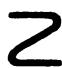
\includegraphics[keepaspectratio]{images/part002_8e27f267.jpg}}

If the extension M is separable over K, it is not necessarily separable over L (cf.~however V, p.~124, Cor. 3). For example, if p is a prime number, the field \(\mathbf{F}_{p}(\mathbf{X})\) of rational fractions in one indeterminate X over \(F_{p}\) is separable over \(F_{p}\) (V, p.~121, Prop. 6) but it is a p-radical algebraic extension of \(\mathbf{F}_{p}(\mathbf{X}^{p})\) ; in particular \(\mathbf{F}_{p}(\mathbf{X})\) is not separable over \(\mathbf{F}_{p}(\mathbf{X}^{p})\) .

Later (V, p.~137 Prop. 5) we shall study the separability of composite extensions.
